\documentclass[12pt,a4paper]{report}
\usepackage{charter}
\usepackage{graphicx}
\renewcommand{\bibname}{References}
\renewcommand{\appendixname}{Appendix}
\renewcommand{\figurename}{Figure}
\renewcommand{\thefootnote}{\ensuremath{\fnsymbol{footnote}}}
\renewcommand{\contentsname}{Table of Contents}
\renewcommand{\listfigurename}{List of Figures}
\def\chaptername{Chapter}
\newtheorem{theorem}{Theorem}
\newtheorem{acknowledgement}[theorem]{Acknowledgement}
\newtheorem{algorithm}[theorem]{Algoritma}
\def\abstractname{\LARGE \textbf{Abstract}}
\leftmarginii=0cm
\usepackage{vmargin}
\setmarginsrb{2.5cm}{2cm}{2.5cm}{2cm}{0mm}{10mm}{0mm}{10mm}
\pagenumbering{roman}
\usepackage{amsmath}
\usepackage{amssymb}
\usepackage{enumitem}
\usepackage{calligra}
\usepackage{tikz}
\usetikzlibrary{shapes,arrows}
\usepackage{fancybox}

\begin{document}
% Title page
\newpage
\renewcommand{\thepage}{\roman{page}}
\setcounter{page}{0}
\begin{center}
\LARGE \textbf{A THEORETICAL STUDY ON A TWO-DIMENSIONAL FLAP-TYPE WAVEMAKER}\\
\vspace{2cm} 
\large \textbf{Final Project}\\ 
\textbf{Proposed as a requirement for an undergraduate degree}\\
\vspace{5cm} 
\large \textbf{by}\\ 
\Large \textbf{Natanael Karjanto}\\ 
\textbf{10197045}\\ 
\vspace{5cm}
\begin{figure}[h]
\begin{center}

\includegraphics[scale = 0.8]{gajah.png}
\end{center}
\end{figure}
\normalsize 
\textbf{DEPARTMENT OF MATHEMATICS} \\ 
\textbf{FACULTY OF MATHEMATICS AND NATURAL SCIENCES} \\ 
\textbf{BANDUNG INSTITUTE OF TECHNOLOGY}\\ 
\textbf{2001}
\end{center}

% Approval page
\newpage
\setcounter{page}{0}
\begin{center}
\LARGE \textbf{A THEORETICAL STUDY ON A TWO-DIMENSIONAL FLAP-TYPE WAVEMAKER}\\
\vspace{0.5 in} \large \textbf{Approval Page}\\ \vspace{1 in}
\Large \textbf{\large It has been examined and approved by the Supervisor:}\\
\vspace{1.25 in} \textbf{\underline{Dr. Andonowati}}\\
\textbf{NIP. 131803263}\\ \vspace{1.5 in} \Large 
\textbf{and Examiners:}
\Large \vspace*{3.2cm}\\
\hspace*{0.5cm}\textbf{\underline{Prof. Dr. M. Ansjar}} \hfill \textbf{\underline{Dr. Wono Setya Budhi}\hspace*{0.5cm}} \\
\hspace*{0.8cm}\textbf{NIP. 130143972} \hfill \textbf{NIP. 131284801} \hspace*{1cm}
\end{center}

% Dedication page
\newpage
\begin{verse}
\setcounter{page}{0}
\vspace*{2cm}
\begin{center}
\emph{For my beloved father, mother, and sister.}
\end{center}
\end{verse}

% English abstract
\begin{abstract}
\setcounter{page}{4}

{\normalsize A mathematical model for unidirectional wave generation explained in this study. The model consists of Laplace's equation in the semi-infinite two-dimensional water interior, dynamic and kinematic boundary conditions at the free surface, lateral boundary condition on the wavemaker, and fixed wall at the bottom. The model is for a flap-type wavemaker that is commonly used in a towing tank of a hydrodynamic laboratory. To simplify the problem, some assumptions are made, namely that water is an ideal fluid. Linear wavemaker theory is used and a generation of monochromatic wave (single frequency) is considered. The relation between the wavenumber, wave height, and wavemaker stroke is further derived. \par} \vspace*{1cm}

\noindent 
{\normalsize \textbf{Keywords:} ideal fluid, wavemaker, Laplace equation, kinematic free surface, dynamic free surface, linear wavemaker theory, monochromatic wave, wavenumber, wave height, and wavemaker stroke. \addcontentsline{toc}{chapter}{Abstract} \par}
\end{abstract}

% Foreword
\begin{center}
\huge {\textbf{Foreword}}
\end{center}
%\baselineskip=0.3 in
\setcounter{page}{6}

\normalsize {\Huge \textbf{T}}hank you to the readers who take the time to open this final project report. First of all, allow me to thank God Almighty for blessing me to complete this project and to finish my undergraduate degree. I am also grateful to the following individuals who have supported me during my study.
\addcontentsline{toc}{chapter}{Foreword}
\begin{enumerate}[leftmargin=1.2em]
\item Dr. Andonowati who was willing and patiently supervised this project.

\item Professor Dr. M. Ansjar and Dr. Wono Setya Budhi who have become the examiners for the project presentation on 15 December 2000. 
I thank Professor Ansjar for trusting me as his teaching assistant in Mathematical Methods during Fall/Autumn 2000.
I am grateful to Dr. Wono for patiently teaching me \emph{Maple} and \LaTeX \ so that this report can be completed nicely.

\item Dr. Nana Nawawi Gaos for being my academic adviser during Common First Year 1997/1998 and Intensive Semester of 1998.

\item Dr. Ahmad Muchlis for being my academic advisor during my sophomore until senior years. Thank you for motivating me to complete my undergraduate study in three and half a year.

\item Warsoma Djohan M.Si. for delegating me as his teaching assistant for Calculus 1 during Fall 1999 and Fall 2000.
I thank Dr. Jalina Widjaja for having me as her teaching assistant in Engineering Mathematics, Matrix and Vector Spaces and Calculus 1 as well as Dr. Nuning Nuraini whom I assist in her Calculus 2 course. I would not forget Koko Martono M.Si. for delegating me as his teaching assistant in Multivariable Calculus and Complex Function as well as training me to write scientific articles. I acknowledge other instructors and professors who have contributed me in developing my mathematical maturity.

\item My parents who have supported me financially and their incessant prayer during my study. My beloved sister who has supported and motivated me to study diligently.

\item Hadi Susanto for being my friend, both in good and bad times, particularly before he departed to the Netherlands. \textsl{Ik wil U bedanken omdat U mij heel goed heeft gemotiveend om extra hard te studeren. Bedankt, Hadi!}

\item Maykel, Luis, Dina, Ety, Sica, Anna, Sondang, Rilyovira and other friends from the Class of 1997 whom I could not mention individually. Thanks for our friendship. I also thank both my seniors and juniors who have assisted me during my study.

\item Toto Nusantara (MA-S3), Lylye Sulaeman (P4M) and Surya (MA96) who have helped me in \TeX, \LaTeX, and \emph{Scientific Work Place} to type this report.

\item Wili (MA97), Henry (FI97), Albert(TF97), Wila (TI97), Aan (TK97), Faiq (TG97), Krshna (EL97), Fitra (TA98), Dindin (TL98), Hidayat (FA98), Dwi Susanti (FA98), Mia (KI99), Erika (FA99), Dwi Hesti (TG2000) and other friends as well as juniors from SMA Negeri 4 Bandung who have motivated and supported me to complete my study in less than eight semesters. I am grateful to you all!
\end{enumerate}

\emph{Experientia est optima rerum magistra} is a well-known Latin expression for ``Experience is the best teacher''. Like other events in life, completing the undergraduate study as well as finishing this report is a unique and interesting experience for me, become a `teacher' in happiness and sorrow. I have learned many things when writing this report, not only academically but also growing mature thinking.

With a humble heart, I am fully aware that as a person, I am merely an individual from a crowd who comes and goes and attempts to imprint an academic achievement at this department and university. Although I might not be able to present my best for the progress of the department, I have striven to do my best in completing this project. I also hope that this `tiny' writing could become \emph{cr\'eme de la cr\'eme} from all the work that I have made albeit there are many limitations in various aspects.

Therefore, I would like to take this opportunity to apologize to the readers of this final project report. I hope this piece of work could be beneficial not only for interested readers but also for the progress of Mathematics.
\begin{flushright}
Bandung, mid-January 2001 \vspace*{0.5cm}\\
{\Large \calligra Natanael Karjanto \ }
\end{flushright}


% Table of contents
\newpage
\pagestyle{headings} \setcounter{page}{9}
\addcontentsline{toc}{chapter}{Table of Contents} \tableofcontents

% List of figures
\newpage
\addcontentsline{toc}{chapter}{List of Figures} \listoffigures

% Chapter 1
\chapter{Introduction}

\pagenumbering{arabic}

% Section 1.1
\section{Background and Problem Formulation}

% Subsection 1.1.1
\subsection{Background}

As a nation progresses, the need for research in science and technology is increasing as well. More than two-thirds of the Indonesian territory consists of seas with abundant natural resources. Indonesia has been known as a maritime nation since ancient times. As science and technology progress, there is a need for research in the maritime area. 

In Ocean Engineering, the need to model phenomena in the open ocean mathematically motivates the research in this area. This leads to interdisciplinary collaboration among various fields of science and engineering. Mathematics as the queen and servant of science has the powerful ability to model many natural phenomena. In this final project report, we will discuss a theoretical study for a wave generation in a towing tank.\footnote[1]{A towing tank is a facility in a hydrodynamic laboratory, the long pond contains water with a wavemaker on one side and a wave absorber on the other side. Some examples are listed in Appendix~C.}

Modeling the wave generation process in a hydrodynamic laboratory is useful for ship testing as if the ship is sailing in the open ocean.
For example, a ship that plans to sail in the Javanese Sea should be tested with the ocean waves characterizing the ones in the Javanese Sea.
Keeping this in mind, we could obtain information on how strong the ocean waves are and this translates to building a strong ship that could handle the pressure from those ocean waves.

% Subsection 1.1.2
\subsection{Problem Formulation}

Based on the above background, we propose a mathematical model for ocean waves using the wavemaker theory utilized in a laboratory.
We would like to investigate how large we should deviate the wavemaker if we wish a wave profile with particular wave height. 
Additionally, we would like to examine the resulting wave profile if we move the wavemaker with a particular frequency.
Hence, we could formulate a mathematical model for water wave evolution in a towing tank.

% Section 1.2
\section{Study Coverage}

Based on the above problem formulation, the study coverage of this report is proposing a simple mathematical model of a two-dimensional flap-type wavemaker in a towing tank.
We will adopt relevant assumptions to simplify the problems. We only consider the output of monochromatic waves. Using computer software, a simple simulation describing the wave evolution will be presented.

% Section 1.3
\section{Purpose}

A subjective purpose of writing this final project report is fulfilling the requirement for completing an undergraduate degree at the Department of Mathematics, Faculty of Mathematics and Natural Sciences, Bandung Institute of Technology. The meeting for the degree conferring was held on 24 January 2001.

An objective purpose of this writing is to deepen the study of Mathematics, particularly its applications in physical problems.
Additionally, by modeling problem from outside Mathematics, the insight regarding the interconnection of science and technology will also be expanded.

% Section 1.4
\section{Basic Assumptions}

The proposed model depends on the following factors:
\begin{itemize}[leftmargin=1.2em]
\item The assumption of fluid characteristics leads to mathematical formulation.
\item There exists a governing differential equation with several boundary conditions.
\item An assumption regarding the type and the characteristics of the output waves.
\end{itemize}

% Section 1.5
\section{Hypothesis}

If we adopt an assumption that water is an ideal fluid, then we could obtain a partial differential equation with several boundary conditions as a governing differential equation. If we also adopt another assumption that the output wave is monochromatic and periodic, then we could propose a linear, two-dimensional wave generation theory.

% Section 1.6
\section{Research Methodology}

% Subsection 1.6.1
\subsection{Methodology}

We implement the theoretical and analytical methodology. This means analyzing theoretically a model related to the wave generation and deriving equations related to this model. We also implement computational analysis methodology to analyze and solve problems using a computer.

% Subsection 1.6.2
\subsection{Data Collection}

Data collection includes literature study and regular meetings with the supervisor. A literature study covers independent learning references related to Fluid Mechanics and Mathematical Modeling, particularly related to wave generation theory. The list of references can be found in the References for this report. The supervising activity includes reading assignments, discussion and problem-solving. Presentations were also conducted regularly. 

% Section 1.7
\section{Discussion Flow}

After this introduction, we will discuss the characteristics of ideal fluid flow. Chapter~\ref{ideal} also explains the physical characteristics of the fluid, the derivation of the continuity equation, Euler's equation, and Bernoulli's equation using the Laws of Mass and Momentum Conservation, as well as using the Transport Theorem. Several assumptions and equations covered in this chapter will be utilized in the subsequent chapters.

Chapter~\ref{wavemaker}, the main part of this report, covers the problem formulation and the study coverage. We will not only discuss the simplified wave generation theory but also more realistic linear theory by solving the Laplace equation as the governing equation with a lateral boundary condition at the wavemaker, a boundary condition at the bottom of the towing tank, and boundary conditions at the surface of the water. The latter includes kinematics and dynamic boundary conditions.

While the theoretical approach and derivation dominate the preceding chapters, Chapter~\ref{numeric} explains computer simulation using {\slshape Maple V Release 5}. We calculate the values of progressive and traveling wavenumbers. We will display some figures related to the movement of the wavemaker and the produced monochromatic wave profiles.

The final chapter concludes this final project report. We also provide practical suggestions for friends and anyone interested to continue research in this area.

% Chapter 2
\chapter{Ideal Fluid Flow}    \label{ideal}

% Section 2.1
\section{Fluid Physical Characteristics}

Due to its ability to move, it is interesting to observe fluids.
A fluid is a substance that does not experience resistance when it experiences deformation and will continue to change when it is given pressures or forces.
It does not have a regular shape and always follows the space it places.
Under the influence of a force, a fluid will deform continually to form a flow.

Fluids can be categorized as liquid and gas. A liquid has a characteristic of relatively incompressible and possesses a free surface.
A gas has a characteristic of readily compressible and does not possess a free surface.
In this chapter, we will discuss liquid fluid, particularly water.
The property of water in our context belongs to the ideal fluid, i.e., incompressible and inviscid fluid.
This choice of assumptions will be used as a fundamental flow problem that we will discuss later~\cite{rs,wlh}.

% Section 2.2
\section{The Laws of Mass and Momentum Conversation}

The laws of conservation for a system of particles in Physics can also be applied to fluids since fluids are a collection of particles.
Based on this, we focus on a collection of fluid particles or a fluid material volume so that we always examine an identical particle group.

For easier symbolic writing, we express the Cartesian coordinates as the index $(1,2,3)$ with a convention that $x = x_{1}$, $y = x_{2}$, and $z = x_{3}$.
The same convention also applies for the velocity components, i.e. $u = u_1$, $v = u_2$, and $w = u_3$.

% Subsection 2.2.1
\subsection{The Law of Conservation of Mass}

The law of conservation of mass states that the total mass of a system composed of a collection of particles is always constant, it neither increases nor decreases.

In other words, there exists no fluid mass that can be created not annihilated.
The change of mass within a domain is due to the mass flow passing through a boundary.
Based on this restriction, we define fluid volume $V(t)$ bounded by a surface $S$.
If the fluid has a density $\rho$, then the total fluid mass in that volume is given by the triple integral
$\iiint \rho \, \mathrm{d}V$. In our formulation, the law of mass conservation states that the total fluid mass with density $\rho$ and volume $V$ is constant.
Stated differently, this law gives a requirement that the triple integral is constant:
\begin{equation}
\iiint\limits_{V} \rho \, \mathrm{d}V = \textmd{constant}
\end{equation}
or
\begin{equation}
\frac{d}{dt} \left(\iiint\limits_{V} \rho \, \mathrm{d}V \right) = 0. \label{ms}
\end{equation}

% Subsection 2.2.2
\subsection{The Law of Conservation of Momentum}

The law of conservation of momentum states that the total momentum of a system composed by a collection of interacting particles is constant, as long as there is no external force acting to the system.

Similarly, the density of fluid-particle momentum is $\rho\,\mathbf{u}$ with components $\rho\,u_{i}$.
In our context, the law of conservation of momentum requires that the total forces acting on a fluid volume equals the rate of change of the fluid momentum.
According to the Newtonian frame of reference, we can express the law of conservation of momentum as follows:
\begin{equation}
\frac{d}{dt}\left(\iiint\limits_{V} \rho \, u_i \, \mathrm{d}V \right) = \iint\limits_{S} \tau_{ij} \; n_{j} \; \mathrm{d}S + \iiint\limits_{V} F_i \, \mathrm{d}V, \label{mt}
\end{equation}
where $\rho\,u_{i}$ denotes the component of fluid particles momentum density, $\tau_{ij}$ denotes the pressure tensor acting on the fluid volume, $n_{j}$ denotes the unit normal vector component on the fluid surface, and $F_{i}$ denotes an external force working on the fluid particles. The surface integral is the $i$-th component from the surface forces acting on the surface $S$ and the final triple integral is the sum from external body force, including the gravitational force.

Using the Divergence Theorem,\footnote[1]{In Western countries, this theorem is known as Gauss Theorem, while in the Eastern Block territory, the theorem is known as Ostrogradsky Theorem, based on the name of one Russian mathematician~\cite{tgb}.} the first term on the right-hand side of~\eqref{mt} can be expressed as a triple integral of a divergence of a vector field covering the corresponding surface
\begin{equation}
\iint\limits_{S} \mathbf{Q}\cdot\mathbf{n} \, \mathrm{d}S = \iiint\limits_{V} \nabla \cdot \mathbf{Q} \, \mathrm{d}V.  \label{tdg}
\end{equation}
Written in component form, this equation can be expressed as
\begin{equation}
\iint\limits_{S} Q_{i} \, n_{i} \, \mathrm{d}S = \iiint\limits_{V} \frac{\partial Q_{i}}{\partial x{i}} \, \mathrm{d}V.  \label{td}
\end{equation}
Here, $\mathbf{Q}$ denotes an arbitrary continuous and differentiable vector field in the volume $V$ and the unit normal vector $\mathbf{n}$ denotes the normal vector going in the outer direction from $V$ on the surface $S$.

Using~\eqref{td} to transform the surface integral to~\eqref{mt}, we obtain
\begin{equation}
\frac{d}{dt}\left(\iiint\limits_{V} \rho \, u_i \, \mathrm{d}V \right) = \iiint\limits_{V} \left(\frac{\partial \tau_{ij}}{\partial x_{j}} + F_{i} \right) \, \mathrm{d}V. \label{tr}
\end{equation}
Equations~\eqref{ms} and~\eqref{tr} express the Laws of Conservation of Mass and Momentum for the fluid integrated over the arbitrary material volume $V(t)$, respectively.

% Section 2.3
\section{Transport Theorem}

Let a general form of the volume integral be expressed as follows:
\begin{equation}
I(t) = \iiint\limits_{V(t)} f(\mathbf{x}, t) \, \mathrm{d}V.
\end{equation}
Here, $f$ denotes an arbitrary differentiable scalar function that depends on the position $\mathbf{x}$ and time $t$ integrated over the volume $V(t)$, for which the latter can also change in time. Hence, the surface $S$ of the volume boundary will change in time as well and its normal velocity is denoted by $U_n$.

Using a common techniques employed in basic Calculus, consider the following difference:
\begin{equation}
\Delta I = I(t + \Delta t) - I(t) = \iiint\limits_{V(t+\Delta t)} f(\mathbf{x}, t + \Delta t) \, \mathrm{d}V - \iiint\limits_{V(t)} f(\mathbf{x}, t) \, \mathrm{d}V. \label{di}
\end{equation}
From the Taylor series of $f(\mathbf{x},t+ \Delta t)$, we have
\begin{equation}
f(\mathbf{x}, t + \Delta t) = f(\mathbf{x}, t) + \Delta t \, \frac{\partial f(\mathbf{x}, t)}{\partial t} + 
                              \frac{1}{2!} \, (\Delta t)^2 \,\frac{\partial^2 f(\mathbf{x}, t)}{\partial t^2} + \cdots.
\end{equation}
Neglecting the terms proportional to the order of $(\Delta t)^2$ and higher, we attain
\begin{equation}
f(\mathbf{x}, t + \Delta t) = f(\mathbf{x}, t) + \Delta t \, \frac{\partial f(\mathbf{x}, t)}{\partial t}.
\end{equation}
We can apply a similar analysis to the material volume $V(t)$
\begin{equation}
V(t + \Delta t) = V(t) + \Delta t \, \frac{dV}{dt} + \frac{1}{2!} \, (\Delta t)^2 \, \frac{d^2V}{dt^2} + \cdots.
\end{equation}
Neglecting the higher-order terms, we obtain
\begin{equation}
\Delta V = V(t + \Delta t) - V(t).
\end{equation}
Thus, $V(t + \Delta t)$ differs from $V(t)$ a thin volume $\Delta V$ included insides the boundary surfaces $S(t + \Delta t)$ and $S(t)$ and is proportional with $\Delta t$.
From~\eqref{di}, we obtain
\begin{align}
\Delta I &= \iiint\limits_{V + \Delta V} \left(f + \Delta t \, \frac{\partial f}{\partial t} \right) \, \mathrm{d}V - \iiint\limits_{V} f \, \mathrm{d}V \\
         &= \Delta t \iiint\limits_{V} \frac{\partial f}{\partial t} \mathrm{d}V + \iiint\limits_{\Delta V} f \, \mathrm{d} V + {\mathcal{O}} \left[(\Delta t)^2 \right],
\end{align}
where the final term denotes the second order error proportional to $(\Delta t)^2$. 

To evaluate the integral over the tiny volume $\Delta V$, we notice that this thin solid has the same thickness as the distance between $S(t)$ and $S(t + \Delta t)$.
This thickness equals to the normal component from the distance covered by $S(t)$ in time $\Delta t$, which is the product $U_n \, \Delta t$.
Thus, the integral of the second term only contributes to the first order, which is proportional to $\Delta t$.
The degree of accuracy of the integrand function $f$ can be assumed to be constant throughout the thin solid in the direction of the normal from the surface $S$.
Integrating only in this direction, we have the following:
\begin{equation}
\Delta I = \triangle t \iiint\limits_{V} \frac{\partial f}{\partial t} \, \mathrm{d}V + \iint\limits_{S} (U_{n} \, \triangle t) \, f \, \mathrm{d}S + 
		   {\mathcal{O}} \left[(\triangle t)^2 \right].
\end{equation}
Finally, we obtain the desired result by dividing both sides of the equation by $\Delta t$ and take the limit by allowing $\Delta t$ approaching zero
\begin{equation}
\frac{\mathrm{d}I}{\mathrm{d}t} = \lim_{\Delta t \rightarrow 0} \, \frac{\triangle I}{\triangle t} = \iiint\limits_{V} \frac{\partial f}{\partial t} \, \mathrm{d}V + 
				\iint\limits_{S} f \, U_{n} \, \mathrm{d}S.  \label{tt}
\end{equation}

Equation~\eqref{tt} is known as the Transport Theorem or the Transport Equation.
The surface integral in this equation states the transport quantity $f$ moving out from the volume $V$ as a result of the moving boundary.
In the special case when $S$ is fixed and $U_n = 0$, equation~\eqref{tt} reduces to a simple form where the differential operator can be pulled out from the integral sign.
For a complete explanation, please consult~\cite{njn}.

We have another interesting case. Since the material volume $V$ is always composed by identical fluid particles, then the surface $S$ moves with the same normal velocity with the one of the fluid itself and $U_{n} = \mathbf{u} \cdot \mathbf{n} = \mathbf{u}_{i} \, \mathbf{n}_{i}$.
In this case, applying the Divergence Theorem to equation~\eqref{tdg}, then we can express equation~\eqref{tt} in the following form:
\begin{align}
\frac{\mathrm{d}I}{\mathrm{d}t} 
&= \frac{\mathrm{d}}{\mathrm{d}t} \left(\iiint\limits_{V(t)} f \, \mathrm{d}V \right) \nonumber \\
&= \iiint\limits_{V(t)} \frac{\partial f}{\partial t} \, \mathrm{d}V + \iint\limits_{S} f\, u_{i} \, n_{i} \, \mathrm{d}S \\
&= \iiint\limits_{V(t)} \frac{\partial f}{\partial t} \, \mathrm{d}V + \iiint\limits_{V(t)} \frac{\partial}{\partial x_{i}} \, \left(f \, u_{i} \right) \, \mathrm{d}V \\
&= \iiint\limits_{V(t)} \left[\frac{\partial f}{\partial t} + \frac{\partial}{\partial x_{i}} \, \left(f \, u_{i} \right) \right] \, \mathrm{d}V.  \label{fdv}
\end{align}

% Section 2.4
\section{Continuity Equation}     \label{kontinuitas}

This equation is closely related to the Law of Conservation of Mass and the Transport Theorem since it can be derived from these two equations.
Look again equation~\eqref{ms} for the Law of Conservation of Mass. Using the result of the Transport Theorem~\eqref{fdv}, we obtain
\begin{equation}
\frac{\mathrm{d}}{\mathrm{d}t} \left(\iiint\limits_{V} \rho \, \mathrm{d}V \right) = \iiint\limits_{V} \left[\frac{\partial \rho}{\partial t} + 
\frac{\partial}{\partial x_{i}} \, \left(\rho \, u_{i} \right) \right] \, \mathrm{d}V = 0.
\label{ce}
\end{equation}
Since the last integral is evaluated at a fixed instantaneous time, the difference that $V$ is material volume is not necessary at this stage.
Furthermore, that particular volume can be composed of a group of arbitrary fluid particles.
Hence, the integrand above is identically zero throughout the whole fluid.
Therefore, the volume integral in~\eqref{ce} can be replaced by a partial differential equation expressing the Law of Conservation of Mass in the following form:
\begin{equation}
\frac{\partial \rho}{\partial t} + \frac{\partial}{\partial x_{i}} \, (\rho \, u_{i}) = 0.
\end{equation}
Written in a three-dimensional component form, this equation reads
\begin{equation}
\frac{\partial \rho}{\partial t} + \frac{\partial \rho u}{\partial x} + \frac{\partial \rho v}{\partial y} + \frac{\partial \rho w }{\partial z} = 0, 	\label{ko}
\end{equation}
or written in a differential form
\begin{equation}
\frac{\partial\rho}{\partial t} + \nabla \cdot (\rho \, \mathbf{u}) = 0.
\end{equation}

This important equation is known as the condition for the Law of Conservation of Mass or the continuity equation for incompressible fluid flow.
Equation~\eqref{ko} describes the mean rate of change of mass density at a fixed point as a result of the change in the mass velocity vector $\rho \, \mathbf{u}$.
By expanding the terms containing the product of density and the velocity components, we can derive a different form of the continuity equation
\begin{align}
\frac{\partial \rho}{\partial t} + u\,\frac{\partial \rho}{\partial x} + \rho\, \frac{\partial u}{\partial x} + v \, \frac{\partial \rho}{\partial y} + 
\rho\,\frac{\partial v}{\partial y} + w \, \frac{\partial \rho}{\partial z} + \rho \,\frac{\partial w}{\partial z} &=0 \\
\left(\frac{\partial \rho}{\partial t} + u \,\frac{\partial \rho}{\partial x} + v\,\frac{\partial \rho}{\partial y} + w\,\frac{\partial \rho}{\partial z} \right) + 
\rho \, \left(\frac{\partial u}{\partial x} + \frac{\partial v}{\partial y} + \frac{\partial w}{\partial z} \right) &=0.  \label{eks}
\end{align}
Using the material or the total derivative operator (See Appendix~A), equation~\eqref{eks} can be written as follows:
\begin{equation}
\frac{D\rho}{Dt} + \rho \, (\nabla \cdot \mathbf{u}) = 0.  \label{mat}
\end{equation}

For a steady flow, i.e., a time-independent flow, it follows that $\frac{\partial \rho}{\partial t} = 0$ and hence the continuity equation reduces to 
$\nabla \cdot(\rho \, \mathbf{u}) = 0$. Using the assumption that water is incompressible fluid, i.e., having a constant mass rate $\rho$, then the continuity equation~\eqref{eks} reduces to
\begin{equation}
\frac{\partial u}{\partial x} + \frac{\partial v}{\partial y} + \frac{\partial w}{\partial z} = 0.
\end{equation}
We obtain the following expression in the vector form, which can also be derived directly from equation~\eqref{mat}:
\begin{equation}
\nabla \cdot \mathbf{u} = 0.  \label{vpk}
\end{equation}
This relationship is known as the condition of incompressibility. This condition states the fact that the balance between outflow and inflow for a volume element or material volume is zero for all time. 

% Section 2.5
\section{Euler's Equation}

While the continuity equation is related to the Law of Conservation of Mass, Euler's equation is related to the Law of Conservation of Momentum and the Transport Theorem since its derivation makes use of these two equations.
Look again equation~\eqref{tr} for the Law of Conservation of Momentum.
Using the result from the Transport Theorem~\eqref{fdv}, we obtain
\begin{equation}
\iiint\limits_{V} \left[\frac{\partial \rho u_{i}}{\partial t} + \frac{\partial}{\partial x_{j}} \, \left(\rho \, u_{i} \,u_{j} \right) \right] \, \mathrm{d}V = 
\iiint\limits_{V} \left(\frac{\partial \tau_{ij}}{\partial x_{j}} + F_{i} \right) \, \mathrm{d}V.  		\label{eu1}
\end{equation}
Since these integrals are calculated over an identical volume, then the equation for the integrand parts of~\eqref{eu1} must be satisfied as well, it is given as follows:
\begin{equation}
\frac{\partial}{\partial t}(\rho \, u_{i}) + \frac{\partial}{\partial x_{j}} \, \left(\rho \, u_{i} \, u_{j} \right) = \frac{\partial \tau_{ij}}{\partial x_{j}} + F_{i}. \label{eu2}
\end{equation}
Next, by expanding the derivatives of the left-hand side of~\eqref{eu2} using the Chain Rule, we obtain
\begin{equation}
u_{i} \frac{\partial \rho}{\partial t} + \rho \frac{\partial u_{i}}{\partial t} + u_{i} u_{j} \frac{\partial \rho}{\partial x_{j}} + 
\rho u_{j} \frac{\partial u_{i}}{\partial x_{j}} + \rho u_{i} \frac{\partial u_{j}}{\partial x_{j}} = \frac{\partial \tau_{ij}}{\partial x_{j}} + F_{i}.
\end{equation}
Using the assumption that the observed fluid is incompressible and possesses constant mass density $\rho$, using the result of the continuity equation~\eqref{vpk}, we obtain Euler's equation,\footnote[1]{Euler, Leonhard (1707-83). \ Swiss mathematician with a calm mind who fundamentally and meaningfully contributed to various branches of mathematics and their applications, including but not limited to, differential equations, infinite series, complex analysis, mechanics and hydrodynamics, as well as calculus of variations. He was also influential in promoting the use and the understanding of analysis.~\cite{jrs}} also known as the momentum equation
\begin{equation}
\frac{\partial u_{i}}{\partial t} + u_{j} \, \frac{\partial u_{i}}{\partial x_{j}} = \frac{1}{\rho} \, \left(\frac{\partial \tau_{ij}}{\partial x_{j}} + F_{i} \right).  \label{tum}
\end{equation}
Using the material derivative operator (see again Appendix A), Euler's equation~\eqref{tum} can be expressed as follows:
\begin{equation}
\frac{\mathrm{D} u_{i}}{\mathrm{D}t} = \frac{1}{\rho} \, \left(\nabla \cdot \tau_{i} + F_{i} \right).
\end{equation}

% Section 2.6
\section{Bernoulli's Equation} 			\label{bernoulli}

Consider again equation~\eqref{tum}. In a frictionless flow, there exists neither shear stress nor normal stress for isotropic fluid flow.
We adopt a convention that the normal stresses $\tau_{11}, \tau_{22}$, and $\tau_{33}$ have positive orientation if they are tensions.
Since we assume that water is inviscid fluid, then the stress tensor $\mathbf{\tau}$ has only the normal components from the pressure.
For further explanation, please consult~\cite{hwf,kjp,njn}. We set as follows
\begin{equation}
\tau_{11} = \tau_{22} = \tau_{33} = -\,p,
\end{equation}
so that the momentum equation becomes
\begin{equation}
\frac{\partial u_{i} }{\partial t} + u_{j} \, \frac{\partial u_{i}}{\partial x_{j}} = \frac{1}{\rho} \, \left(\frac{\partial p}{\partial x_{j}} + F_{i} \right),
\end{equation}
or in a vector notation
\begin{equation}
\frac{\mathrm{D} \mathbf{u}}{\mathrm{D}t} = \frac{1}{\rho} \, \left(-\nabla p + \mathbf{F} \right),
\end{equation}
where $\mathbf{u} = (u,\,v,\,w)$, \ $\mathbf{F} = (0,\, 0,\, -\rho \,g)$, and $p$ is the pressure. Hence,
\begin{equation}
\frac{\partial \mathbf{u}}{\partial t} + (\mathbf{u} \cdot \nabla) \, \mathbf{u} = -\nabla \, \left(\frac{p}{\rho} + g \,z \right).
\end{equation}
From a vector identity, we have
\begin{equation}
\mathbf{u} \times (\nabla \times \mathbf{u}) = (\mathbf{u} \cdot \nabla) \, \mathbf{u} - \nabla \, \left(\frac{1}{2} \left|\mathbf{u} \right|^2 \right).
\end{equation}
If we also assume that water is irrotational fluid,\footnote[1]{Irrotational fluid in this context refers to the absence of eddy or whirlpool.}, then $\nabla \times
\mathbf{u} = \mathbf{0} \label{curl}$, and thus $(\mathbf{u} \cdot \nabla) \, \mathbf{u} = \nabla \, \left(\frac{1}{2} \left|\mathbf{u} \right|^2 \right)$.
Due to this assumption, the vector velocity $\mathbf{u}$ can be expressed as the gradient of the scalar or velocity potential, i.e., $\mathbf{u} = \nabla\,\phi$.
(For a detailed explanation, please see~\cite{drg} and~\cite{lld}.) The reason we implemented this simplification is for easier analysis since in general, scalar quantities are less complicated to investigate than vector quantities.

Therefore,
\begin{equation}
\frac{\partial \, \nabla \phi}{\partial t} + \nabla \, \left(\frac{1}{2} \left|\mathbf{u} \right|^2 \right) = -\nabla \, \left(\frac{p}{\rho} + g\,z \right),
\end{equation}
or
\begin{equation}
\nabla \, \left(\frac{\partial \phi}{\partial t} + \frac{1}{2} \left|\mathbf{u} \right|^2 + \frac{p}{\rho} + g\,z \right) = 0.  \label{ber1}
\end{equation}
If we integrate equation~\eqref{ber1} throughout the entire space, then we will obtain Bernoulli's equation\footnote[7]{Bernoulli, Daniel (1700-82). \ This Dutch-born scientist is a member of a famous Swiss family who consists of ten mathematicians (fathers, sons, uncles, cousins). He is well-known for his works on fluid flow and the kinetic theory of gases. His equation for fluid flow was first published in 1783. He also pursued the study and research of astronomy and magnetism and was the first scientist who solved the Riccati equation~\cite{jrs}.} 
\begin{equation}
\frac{\partial \phi}{\partial t} + \frac{1}{2} \left|\mathbf{u} \right|^2 + \frac{p}{\rho} + g\,z = \textmd{constant} \equiv f(t).  \label{ber2}
\end{equation}
\newpage
%\vspace*{-0.5cm}
\tikzstyle{cloud} = [draw = red!50, ellipse, fill=red!30, text width=4.5cm, line width=1.0mm, minimum height=3em]
\tikzstyle{block} = [rectangle, draw = blue!50, fill=blue!30, text width=6cm, text centered, rounded corners, line width=1.0mm, minimum height=3em]
\tikzstyle{trap} = [trapezium, draw = green!80!blue, trapezium right angle = 117, fill=green!40, text width=6.5cm, text centered, rounded corners, line width=1.0mm, minimum height=3em]
\tikzstyle{line} = [draw, very thick, -latex']
\begin{center}
A schematic diagram for an ideal fluid interconnectivity. \vspace*{0.5cm} \\
\begin{tikzpicture}[auto, node distance=2cm,>=latex']
% Place nodes
\hspace*{1cm}
\node [cloud](mass){\sffamily Mass Conservation Law};
\node [block, right of=mass, node distance = 8cm](momentum){\sffamily Momentum Conservation Law};
\hspace*{-4cm} \node [trap, below of=momentum, node distance = 2.5cm](transport){\sffamily Transport Equation};
\hspace*{ 4cm} \node [cloud, below of=mass, node distance = 5cm](continuity){\sffamily \quad Continuity equation};
\node [block, right of=continuity, node distance = 8cm](euler){\sffamily Euler's equation};
\node [block, below of=euler, node distance = 2.5cm](bernoulli){\sffamily Bernoulli's equation};
% Draw edges
%\path [line,dashed] (mass) -- node {$+$} (transport);
\path [line,dashed] (momentum) -- node {$+$} (transport);
%\path [line] (transport) -- (continuity);
\path [line] (transport) -- (euler);
\path [line] (euler) -- (bernoulli);
\draw [->, very thick, dashed] (0,-0.7cm) -- node {$+$} (0,-1.8cm);
\draw [->, very thick] (0,-3.15cm) -- (0,-4.3cm);
\end{tikzpicture}
\end{center}

% Bab 3
\chapter{Two-Dimensional Wavemaker Theory}   \label{wavemaker}

In this chapter, we are going to compare two wavemaker theories in which the corresponding mathematical models have been proposed and investigated. The first part is a simplified theory. A basic idea comes from a displaced volume of water by a flap-type wavemaker in a towing tank. The second part covers a more detailed theory for the flap-type wavemaker. From these two theoretical approaches, we will observe the ratio between the wave amplitude~$H$ with the maximum stroke of the wavemaker~$S$.

In the context of this report, the more detailed theory is based on the linear wave theory developed by Airy\footnote[1]{Airy, Sir George Biddle (1801--1892). \ English mathematician and physicist, who became a Royal Astronomer for 46 years. He contributed not only to the theory of light and astronomy but also to gravity, magnetism, sound, wave propagation, and tidal wave~\cite{jrs}.} around 160 years ago, when he analyzed the behavior of ocean waves~\cite{aph}.

% Section 3.1
\section{Simplified Wavemaker Theory}

For shallow-water waves, simple theory for the propagation of a wave profile produced by a wavemaker was first developed by Galvin in 1964. He reasoned that the displaced water by a wavemaker equals the volume of the top part from the propagated wave. Consider a flap-type wavemaker with a fixed bottom end and possesses a maximum stroke~$S$. The water depth in the towing tank is~$h$. The displaced water volume by the flap deviation is $\frac{1}{2}\,S\,h$. See Figure~\ref{flapscheme}. Meanwhile, the top part of water volume is $\int_{0}^{\frac{1}{2}\,L} \frac{1}{2}\,H \sin (k\,x) \, \mathrm{d}x$, where $k = 2\pi/L$ is the wavenumber. Hence,
\begin{align}
\int_{0}^{\frac{1}{2}\,L} \frac{1}{2} H \sin (k\,x) \, \mathrm{d}x
&= \int_{0}^{\frac{1}{2}\,L} \frac{1}{2} H \sin \left(\frac{2\, \pi}{L} x \right) \, \mathrm{d}x \\ 
&= \frac{H\,L}{2\,\pi } \\ 
&= \frac{H}{k}
\end{align}
By equating the two volumes, we have
\begin{equation*}
\frac{1}{2}\,S\,h = \frac{H}{k} = H\,\frac{L}{2\,\pi} = \frac{H}{2} \left(\frac{L}{2} \right) \, \frac{2}{\pi}
\end{equation*}
where the factor $2/\pi$, also known as the area factor, indicates the ratio between the area formed by the wave profile with the rectangle circumscribed it. From the relationship $\frac{1}{2}\,S\,h = \frac{H}{k}$, we can find out the ratio between the wave height~$H$ and the stroke~$S$, namely
\begin{equation*}
\frac{H}{S} = \frac{1}{2} \,k\,h.
\end{equation*}
This relationship is only valid for the shallow-water waves, i.e., for $ k\,h < \frac{1}{10}\pi$.
\begin{figure}[h]
\begin{center}
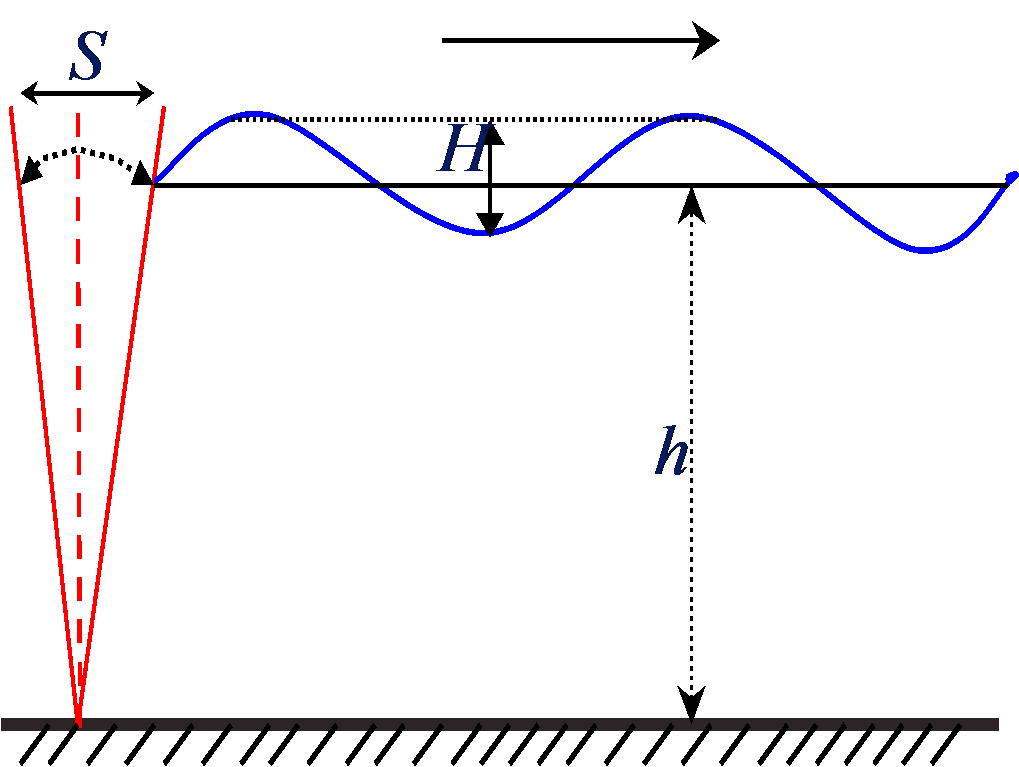
\includegraphics[scale = 3]{skema.png}
\end{center}
\caption{A schematic diagram for a flap-type wavemaker.}             \label{flapscheme}
\end{figure}

% Section 3.2
\section{Linear Wavemaker Theory}

According to the assumption that water is an incompressible fluid, then from the result of equation~\eqref{vpk} in Section~\ref{kontinuitas}, we have $\nabla \cdot \mathbf{u} = 0$. Additionally, another adopted assumption is the absence of water whirlpool, in other words, the water flow is irrotational. Based on this assumption, from the explanation in Section~\ref{bernoulli}, we have obtained $\mathbf{u} = \nabla\,\phi$. Combining these two equations, we obtain $\nabla \cdot \nabla \,\phi = \nabla^{2}\phi = 0$. This equation is known as Laplace's equation\footnote[1]{Laplace, Marquis Pierre Simon de (1749-1827). \ French mathematical-physicist who contributed to the study of celestial mechanics, particularly in explaining the orbit of planets Jupiter and Saturn. He also developed an idea in using potential and orthogonal functions, as well as introduced their integral transformations. He also played an important role in the development of probability theory.}, and it plays a role as a governing differential equation for the velocity potential $\phi$. In the two-dimensional Cartesian coordinates--the $x$- and $z$-axes in the horizontal and vertical directions, respectively--Laplace's equation can be written as follows:
\begin{equation}
\nabla^2\phi = \frac{\partial^2\phi}{\partial x^2} + \frac{\partial^2\phi}{\partial z^2} =0,
\end{equation}
and it is valid for $-h \leq z \leq \eta(x,t)$, and $0 \leq x \leq \infty$.

The boundary value problem in this context is the one for two-dimensional wave propagation in an ideal fluid. We will solve the problem using several boundary conditions that are suitable for the situation in the towing tank. We have at least three boundary conditions as auxiliary equations in solving the governing equation. What follows is the boundary conditions related to the physical condition of the towing tank.

% Subsection 3.2.1
\subsection{Lateral boundary condition at the wavemaker\\ (\emph{pseudo-boundary})}

Let the function describing a horizontal movement at the wavemaker surface be given as follows:
\begin{equation}
F(x,\,z,\,t) = x - \frac{1}{2} \, S(z) \, \sin (\omega \, t) = 0,
\end{equation}
then by applying a total differential to $F(x,\,z,\,t)$, we obtain
\begin{equation}
\frac{\mathrm{D}F}{\mathrm{D}t} = \frac{\partial F}{\partial t} + \frac{\partial F}{\partial x} \frac{\mathrm{d}x}{\mathrm{d}t} + \frac{\partial F}{\partial z} \frac{\mathrm{d}z}{\mathrm{d}t} 
\end{equation}
\begin{align}
%\frac{\mathrm{D}F}{\mathrm{D}t} &= \frac{\partial F}{\partial t} + \frac{\partial F}{\partial x} \frac{\mathrm{d}x}{\mathrm{d}t} + \frac{\partial F}{\partial z} \frac{\mathrm{d}z}{\mathrm{d}t} \\
0 &= -\frac{1}{2} \, \omega \, S(z) \, \cos (\omega \, t) + v - \frac{1}{2} \, w \, \frac{\mathrm{d}S(z)}{\mathrm{d}z} \, \sin (\omega \, t) \\
v - \frac{1}{2} \, w \, \frac{\mathrm{d}S(z)}{\mathrm{d}z} \, \sin (\omega \, t) &= \frac{1}{2} \, \omega \, S(z) \, \cos (\omega \, t) \qquad 
\textmd{on} \quad F(x,\,z,\,t) = 0   \label{phix}
\end{align}
where $v$ and $w$ are the velocity components in the $x$ and $z$ directions, respectively. (Remember that $\mathbf{u} = (v, w)$ is the two-dimensional velocity vector.)
Equation~\eqref{phix} can also be written as follows:
\begin{equation}
\phi_{x} = \frac{1}{2} \left[\phi_{z} \,S\,^{\prime}(z) \, \sin (\omega\, t) + \omega \, S(z) \, \cos \: (\omega\, t) \right].
\end{equation}

For the sufficiently small stroke movement $S(z)$ and stroke velocity, we could linearize equation~\eqref{phix} by neglecting the second term of the left-hand side. Similar to what is applied to a free surface, we can express conditions at the moving lateral boundary in terms evaluated at the mean position, i.e., at $x = 0$. We proceed it by expanding the condition as a truncated Taylor series, or more precisely, in a truncated Maclaurin series
\begin{align}
\displaystyle \left. \left(\phi_{x} - \frac{1}{2} \, \omega \, S(z) \, \cos (\omega\,t) \right) \right|_{x = \frac{1}{2} \, S(z) \, \sin (\omega\,t)} = \left.\left(\phi_{x} - \frac{1}{2} \, \omega \, S(z) \, \cos (\omega\, t) \right) \right|_{x=0} & \nonumber \\
+ \frac{1}{2} \, S(z) \, \sin (\omega\,t) \, \frac{\partial}{\partial x} \left. \left(\phi_{x} - \frac{1}{2} \, \omega \, S(z) \, \cos (\omega\, t) \right) \right|_{x=0} & + \dots.
\end{align}
It should be obvious that only the first term from the above expansion is linear in $\phi_{x}$ and $S(z)$, while other terms can be neglected since they are assumed to be tiny. Therefore, the final lateral boundary condition as a consequence of the linearization process is the following equation:
\begin{equation}
u(0,\,z,\,t) = \phi_{x} = \frac{1}{2} \, \omega \, S(z) \, \cos(\omega t).
\end{equation}

% Subsection 3.2.2
\subsection{Boundary condition at the bottom of the towing tank (kinematic condition)}

Since there is no water flowing through the bottom of the towing thank, then the fluid velocity in the vertical direction at the bottom is zero
\begin{equation}
\phi_{z} = \frac{\partial\phi}{\partial z} = 0, \qquad \textmd{at} \quad z = -h.
\end{equation}

% Subsection 3.2.3
\subsection{Boundary conditions at the water surface}

\begin{itemize}[leftmargin=1.2em]
\item \textbf{Free-surface kinematic boundary condition}
\end{itemize}

At every boundary, irrespective of whether it is free, such as at the water surface, or fixed, such as at the bottom of a pond, the fluid velocity must satisfy a number of physical requirements. Under the influence of a force, this boundary might experience a deformation. All requirements which act upon the water particle kinematics are known as kinematics boundary conditions. At each fluid surface or interface, there exists no flow passing through the interface, otherwise, the interface itself does not exist in the first place. This occurrence is obvious for the case of an impermeable fixed surface, such as a sheet pile seawall~\cite{drg}.

Let the water surface function be given as follows:
\begin{equation}
G(x,\,z,\,t) = z - \eta(x,\,t) = 0,
\end{equation}
where $\eta(x,\,t)$ denotes the wave elevation, also known as the water surface elevation, which indicates the distance of a point in a wave surface from the mean free surface.
Then, the total differential of the above function gives  
\begin{align}
\frac{\mathrm{D}G}{\mathrm{D}t} &= \frac{\partial G}{\partial t} + \frac{\partial G}{\partial x} \, \frac{\mathrm{d}x}{\mathrm{d}t} + \frac{\partial G}{\partial z} \, \frac{\mathrm{d}z}{\mathrm{d}t} \\
0 &= -\frac{\partial \eta}{\partial t} + \left(-\frac{\partial \eta}{\partial x} \right) \,v + w
\end{align}
or
\begin{equation}
\eta_{t} = w - v \,\eta_{x}.  \label{eta}
\end{equation}
Since $\mathbf{u} = (v,\,w)= (\phi_{x}, \phi_{z}) = \nabla \phi$, then equation~\eqref{eta} can be written as follows:
\begin{equation}
\eta_{t} = \phi_{z} - \phi_{x} \,\eta_{x}.
\end{equation}

Now define $\varphi(x,\,t)= \left. \phi(x,\,z,\,t)\right|_{z=\eta(x,\,t)} = \phi(x,\,\eta(x,\,t),\,t)$. By differentiating it with respect to $x$, we now have $\displaystyle \frac{\partial\varphi}{\partial x} = \frac{\partial\phi}{\partial x} + \frac{\partial\phi}{\partial\eta} \,\frac{\partial\eta}{\partial x}$. We write a notation $\frac{\partial \phi}{\partial \eta} = \gamma$. Hence, this equation becomes $\varphi_{x} = \phi_{x} + \gamma\,\eta_{x}$. By substituting $\phi_{\eta} = \frac{\partial \phi}{\partial \eta} = \gamma$ dan $\phi_{x} = \varphi_{x} - \gamma \,\eta_{x}$ to the equation above we obtain the following equation
\begin{align}
\eta_{t} &= \gamma - \left(\varphi_{x} - \gamma\, \eta_{x} \right) \, \eta_{x} = \gamma - \varphi_{x} \,\eta_{x} + \gamma \, \eta_{x}^2 \\
\eta_{t} &= \left(1 + \eta_{x}^2 \right) \, \gamma - \varphi_{x} \,\eta_{x}.
\end{align}
This is the free surface kinematic boundary condition, a condition that states the fact that there is no fluid particle passes through the free surface.

\begin{itemize}[leftmargin=1.2em]
\item \textbf{Free-surface dynamic boundary condition}
\end{itemize}

A ``free'' water surface, such as the interface between air and water, cannot sustain the pressure difference along the boundary and thus must respond to receive a uniform pressure. Dynamic boundary condition describes a pressure distribution that acts upon the boundaries such as free surface and interface.

From Bernoulli's equation for unsteady flow, we already have the equation $\displaystyle \frac{\partial \mathbf{u}}{\partial t} + \nabla \left(\frac{p}{\rho} + g\,z + \frac{1}{2} \left|\mathbf{u}\right|^2 \right) = 0$. By assuming that the free atmospheric pressure above the water layer bounded by only the free surface, this equation can be written as follows:
\begin{equation}
\frac{\partial {\phi}}{\partial t} + g\,\eta + \frac{1}{2} \left|\nabla \phi \right|^2 = 0, \qquad \textmd{at} \quad z = \eta(x,\,t).  \label{bernou}
\end{equation}

We first calculate $\frac{1}{2} \left|\nabla \phi \right|^2$ to find out its representation in the form of its partial derivatives. We also know that 
\begin{align}
\frac{1}{2} \left|\nabla \phi \right|^2 
&= \frac{1}{2} \, \left(\nabla \phi \cdot \nabla \phi \right) 
 = \frac{1}{2} \, \left[\,\left(\phi_{x}, \, \phi_{z} \right) \cdot \left(\phi_{x}, \, \phi_{z} \right) \,\right]  \nonumber \\
&= \frac{1}{2} \, \left(\phi_{x}^2 + \phi_{z}^2 \right) = \frac{1}{2} \,\left(\phi_{x}^2 + \gamma^2 \right).
\end{align}
By substituting $\phi_{x} = \varphi_{x} - \gamma \, \eta_{x}$ to this equation, we arrive at 
\begin{align}
\frac{1}{2} \left|\nabla \phi \right|^2 
&= \frac{1}{2} \left[\left(\varphi_{x} - \gamma \, \eta_{x} \right)^2 + \gamma^2 \right]  \nonumber \\
&= \frac{1}{2} \left(\varphi_{x}^2 - 2 \gamma \, \varphi_{x} \, \eta_{x} + \gamma^2 \, \eta_{x}^2 + \gamma^2 \right).
\end{align}
Thus, $\displaystyle \frac{1}{2} \left|\nabla \phi \right|^2 = \frac{1}{2} \, \varphi_{x}^2 - \gamma \, \varphi_{x} \, \eta_{x} + \frac{1}{2} \,\left(1 + \eta_{x}^2 \right) \, \gamma^2$.

From $\varphi(x,\,t) = \phi(x, \, \eta(x,\,t), \,t)$, a partial differentiation with respect to $t$ gives $\displaystyle \frac{\partial \varphi}{\partial t} =
\frac{\partial\phi}{\partial t} + \frac{\partial\phi}{\partial\eta} \frac{\partial\eta}{\partial t}$ \quad $\Longrightarrow$ \quad $\varphi_{t} = \phi_{t} +
\gamma \,\eta_{t}$ \quad $\Longrightarrow$ \quad $\phi_{t} = \varphi_{t} - \gamma\,\eta_{t}$.

Substituting to Bernoulli's equation~\eqref{bernou} yields
\begin{equation}
\varphi_{t} - \gamma\,\eta_{t} + \frac{1}{2}\,\varphi_{x}^2 - \gamma \,\varphi_{x} \, \eta_{x} + \frac{1}{2}\,\left(1 + \eta_{x}^2 \right) \,\gamma^2 + g\,\eta = 0.
\end{equation}
To obtain a simplified form, we substitute $\eta_{t} = \left(1 + \eta_{x}^2 \right) \,\gamma - \varphi_{x}\,\eta_{x}$ which is obtained from the kinematic boundary condition. Consequently,
\begin{align}
%\begin{equation}
\varphi_{t} - \gamma\, \left[\left(1 + \eta_{x}^2 \right) \,\gamma - \varphi_{x}\,\eta_{x} \right] + \frac{1}{2}\,\varphi_{x}^2 - \gamma\,\varphi_{x}\,\eta_{x} + \frac{1}{2}\,\left(1 + \eta_{x}^2 \right) \,\gamma^2 + g\,\eta &= 0 \\
%\end{equation}
%\begin{align}
\varphi_{t} - \left(1 + \eta_{x}^2 \right) \,\gamma^2 + \varphi_{x}\,\eta_{x}\,\gamma + \frac{1}{2}\,\varphi_{x}^2 - \gamma\,\varphi_{x}\,\eta_{x} + \frac{1}{2} \,\left(1 + \eta_{x}^2 \right) \,\gamma^2 + g\,\eta &= 0 \\
\varphi_{t} - \frac{1}{2} \,\left(1 + \eta_{x}^2 \right) \,\gamma^2 + \frac{1}{2} \,\varphi_{x}^2 + g\,\eta &= 0.
\end{align}
Finally, we obtain $\displaystyle \varphi_{t} = \frac{1}{2} \,\left(1 + \eta_{x}^2 \right) \,\gamma^2 -\frac{1}{2} \,\varphi_{x}^2 - g\,\eta$. This equation is known as the free surface dynamic boundary condition.

For shallow-water wave, we are more interested in studying and using the linearized form of the free surface kinematic and dynamic boundary conditions since these simplify the problem when we solve the governing differential equations with the prescribed boundary conditions.

Consider again equation~\eqref{eta} as the free surface kinematic boundary condition
\begin{equation}
\frac{\partial \eta}{\partial t} =  w \, \bigg|_{z = \eta} - \frac{\partial \eta}{\partial x} \, (v) \bigg|_{z=\eta}
\end{equation}
or
\begin{equation}
\frac{\partial \eta}{\partial t} = \left. \left(\frac{\partial \phi}{\partial z} \right) \right|_{z = \eta} - \frac{\partial \eta}{\partial x} \, \left. \left(\frac{\partial \phi}{\partial x} \right) \right|_{z = \eta}.
\end{equation}
Neglecting the nonlinear terms, we obtain a simplified form of the free surface kinematic boundary condition, given as follows:
\begin{equation}
\left. \left(\frac{\partial \phi}{\partial z} \right) \right|_{z = 0} = \frac{\partial\eta}{\partial t}.
\end{equation}
Similarly, we also have a simplified form of the free surface dynamic boundary condition, given as follows:
\begin{equation}
\left. \left(\frac{\partial \phi}{\partial t} \right) \right|_{z = 0} = -g \,\eta. 			\label{permukaan}
\end{equation}

A schematic diagram for a wavemaker with a governing equation and its boundary conditions is displayed in Figure~\ref{wavemakerscheme}.
\begin{figure}[h]
\begin{center}
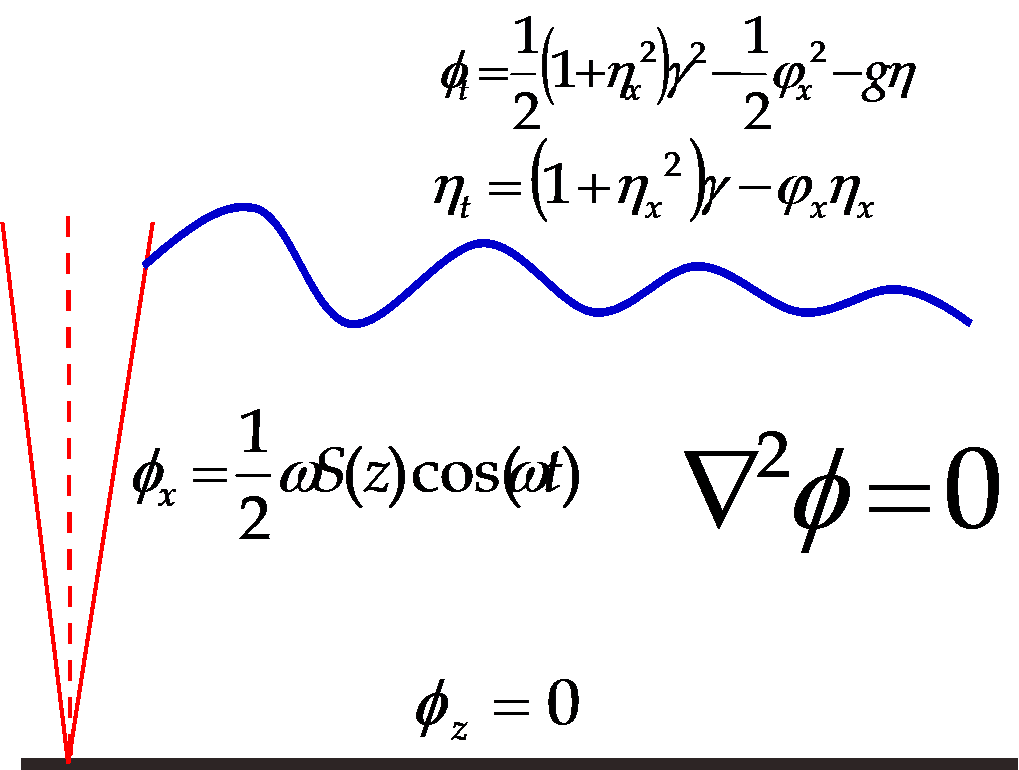
\includegraphics[scale = 3]{governing.png}
\end{center}
\caption{A schematic diagram for a wavemaker with a governing equation and its boundary conditions.}                 \label{wavemakerscheme}
\end{figure}

% Section 3.3
\section{Solutions for the Governing Differential Equation}

The following is an Ansatz for the general solution of velocity potential $\phi$
\begin{align}
\phi(x,\,z,\,t) &= A_{p} \: \cosh \, k_{p}\,(h+z) \: \sin\,(k_{p}\,x - \omega\,t) + (A\,x + B) \nonumber \\
& \quad + C \: e^{-k_{s}\,x} \: \cos k_{s}\,(h + z) \: \cos \, (\omega\, t).   \label{ansatz}
\end{align}
For wavemaker problem, the coefficient $A$ above must equal to zero since there exists no possible uniform flow through the wavemaker and we can also set the coefficient $B$ to be zero as well without influencing the velocity field. The remainder terms must satisfy the two linearized free surface boundary conditions.
It would also be useful to combine these two boundary conditions to a simpler form.
\begin{figure}[h]
\begin{center}
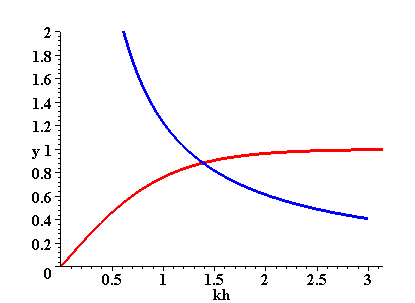
\includegraphics[scale = 0.8]{progresif.png}
\end{center}
\caption[A graph for the progressive wave dispersion relationship.]{A graph for the progressive wave dispersion relationship. This graph illustrates a single root $k_{p}\,h$. The horizontal axis label \textbf{kh} indicates $k_{p}\,h$.}
\label{gambar2}
\end{figure}

Deriving $\phi$ with respect to $t$, we obtain
\begin{equation}
\frac{\partial\phi}{\partial t} = -\, \omega \, A_{p} \: \cosh \, k_{p} \,(h + z) \: \cos \,(k_{p}\,x - \omega\, t) 
- \, \omega \, C \, e^{-k_{s}\,x} \: \cos k_{s}\,(h + z) \:\sin (\omega\, t).
\end{equation}
The second derivative of $\phi$ with respect to $t$ yields
\begin{align}
\frac{\partial^2 \phi}{\partial t^2} &= -\,\omega^2 \, A_{p} \: \cosh \,k_{p} \,(h + z) \: \sin \,(k_{p}\,x - \omega\, t)
- \, \omega^2 \, C \, e^{-k_{s}\,x} \: \cos k_{s} \, (h + z) \: \cos \, (\omega\, t) \nonumber \\
&= -\,\omega^2\,\phi.
\end{align}
From the free surface kinematic and dynamic boundary conditions, we have
\begin{equation}
\frac{\partial \eta}{\partial t} = -\,\frac{1}{g} \, \frac{\partial^2 \phi}{\partial t^2} = -\, \frac{\omega^2}{g}\,\phi = -\,\frac{\partial \phi}{\partial z}, \qquad \textmd{at} \quad z = 0,
\end{equation}
or
\begin{equation}
\frac{\partial \phi}{\partial z} - \frac{\omega^2}{g} \,\phi = 0, \qquad \textmd{at} \quad z = 0.
\end{equation}
By substituting the Ansatz~\eqref{ansatz} to this equation, we obtain
\begin{equation}
\omega^2 = g \, k_{p} \: \tanh \left(k_{p}\,h \right)	  \label{progresif}
\end{equation}
and
\begin{equation}
\omega^2 = -g \, k_{s} \: \tan \left(k_{s}\,h \right).  \label{berdiri}
\end{equation}
The former~\eqref{progresif} is a dispersion relationship for the progressive wave. By rewriting this equation as follows:
\begin{equation}
\frac{\omega^2\,h}{g\,k_{p}\,h} = \tanh \left(k_{p}\,h \right)
\end{equation}
and sketch each term with respect to $k_{p}\,h$ for a particular value of $\displaystyle \frac{\omega^2\,h}{g}$, then we are able to discover the solution for the dispersion relationship~\eqref{progresif} as depicted in Figure~\ref{gambar2}.

The latter~\eqref{berdiri}, which relates $k_{s}$ with the wavemaker frequency $\omega$, determines the wavenumber for the standing wave with an amplitude decaying exponentially as it travels far away from the wavemaker. By rewriting this equation as follows:
\begin{equation}
\frac{\omega^2 \, h}{g \, k_{s} \, h} = -\tan \left(k_{s}\,h\right)
\end{equation}
we can sketch its graph and observe that it possesses an infinite numbers of solution. The solutions of this problem can be observed from the graph for its dispersion relationship, as depicted in Figure~\ref{gambar3}.
\begin{figure}[h]
\begin{center}
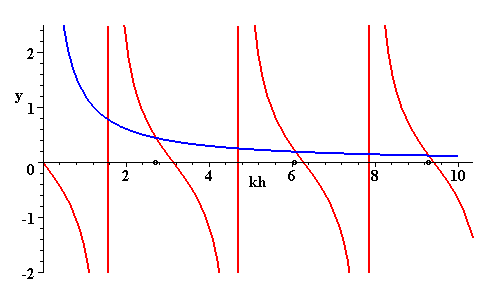
\includegraphics[scale = 0.8]{standing.png}
\end{center}
\caption[A graph for the standing wave dispersion relationship.]{A graph for the standing wave dispersion relationship. This graph illustrates infinitely many compound roots $k_{s}(n)\,h$. The horizontal axis label \textbf{kh} means $k_{s}\,h$.} 				\label{gambar3}
\end{figure}

Each solution is expressed in terms of $k_{s}(n)$, where $n \in \mathbb{N}$. The final form for the velocity potential is given as follows:
\begin{align}
\phi(x,\,z,\,t) &= A_{p} \: \cosh \, k_{p}\,(h + z) \: \sin \,(k_{p}\,x - \omega\,t) \nonumber \\
& \quad + \, \sum_{n = 1}^{\infty} C_{n} \: e^{-k_{s}(n) \, x} \: \cos \, k_{s}(n)\,(h + z) \: \cos (\omega \,t).  \label{lastpotensial}
\end{align}
The first term indicates the progressive wave produced by the wavemaker, while the series terms expresses decaying standing waves as they travel far away from the wavemaker.

To obtain a complete wave solution, we need to determine the coefficients $A_{p}$ and $C_{n}$. We can calculate these values using the wavemaker lateral boundary condition, namely
\begin{equation}
u(0,\,z,\,t) = \left. \left(\frac{\partial \phi}{\partial x} \right) \right|_{x = 0} = \frac{1}{2} \: \omega \, S(z) \: \cos (\omega\,t).
\end{equation}
By finding the first derivative of velocity potential $\phi$ with respect to $x$ and evaluating it at $x = 0$, we attain
\begin{align}
\frac{1}{2} \: \omega \,S(z) \: \cos (\omega\,t) &= A_{p} \, k_{p} \: \cosh \, k_{p}\,(h + z) \: \cos (\omega\,t) \nonumber \\
& \quad - \, \sum_{n = 1}^{\infty} C_{n} \, k_{s}(n) \: \cos \, k_{s}(n) \,(h + z) \: \cos (\omega \,t)
\end{align}
or
\begin{equation}
\frac{1}{2} \: \omega \, S(z) = A_{p} \, k_{p} \: \cosh \, k_{p}\,(h + z) - \sum_{n = 1}^{\infty} C_{n} \, k_{s}(n) \: \cos \, k_{s}(n) \,(h + z).  \label{fourier}
\end{equation}
We now possess a function in the $z$-variable which equals to a series of trigonometric functions on the right-hand side, a situation similar to a Fourier series.
We also have the fact that the set of functions $\left\{ \cosh \,k_{p}\,(h + z), \; \cos \left[ k_{s}(n)\,(h + z) \right] \right \}_{n = 1}^{\infty}$ forms a complete harmonic series orthogonal functions. Any arbitrary continuous function can be expanded in terms of the series.

To find the coefficients $A_p$, therefore, we multiple the above equation with $\cosh \,k_{p} \,(h + z)$ and integrate it with respect to the variable $z$ from $-h$ until $0$. We now acquire
\begin{align}
\int_{-h}^{0} \: \frac{1}{2} \: \omega \, S(z) & \cosh \, k_{p} \,(h + z) \, \mathrm{d}z 
= \int_{-h}^{0} \: A_{p} \, k_{p} \: \cosh \, k_{p}^2 \,(h + z) \, \mathrm{d}z \nonumber \\
&- \int_{-h}^{0} \; \sum_{n = 1}^{\infty} C_{n} \, k_{s}(n) \: \cos \left[k_{s}(n) \, (h + z) \right] \: \cosh \,k_{p}\,(h + z) \, \mathrm{d}z.
\end{align}
Applying the orthogonality property, the last term vanishes and consequently
\begin{equation}
A_{p} = \frac{\displaystyle \frac{1}{2} \: \omega \: \int_{-h}^{0} \: S(z) \: \cosh \, k_{p} \,(h + z) \, \mathrm{d}z}
{\displaystyle k_{p} \: \int_{-h}^{0} \: \cosh \,k_{p}^2 \, (h + z) \,dz}.
\end{equation}
For a flap-type wavemaker, the stroke function $S$ can be specifically expressed as follows:
\begin{equation}
S(z) = S \, \left(1 + \frac{z}{h} \right).
\end{equation}
Employing a simple calculus, we could express the coefficient $A_{p}$ explicitly without the integral sign, given as follows:
\begin{equation}
A_{p} = \frac{2 \, \omega \, S}{k_{p}^2\,h} \; \frac{k_{p} \, h \: \sinh \,k_{p} \,h - \cosh \,k_{p}\,h + 1}{\sinh \, 2 \, k_{p} \, h + 2 \,k_{p} \,h}.  \label{firstconst}
\end{equation}

Similarly, we can obtain the coefficient $C(n)$ by multiplying~\eqref{fourier} with $\cos \,[k_{s}(n) \, (h + z)]$ and integrate it with respect to the variable $z$ over the water depth from $z = -h$ until $z = 0$. We attain
\begin{equation}
C_{n} = \frac{\displaystyle -\frac{1}{2} \: \omega \: \int_{-h}^{0} \: S(z) \: \cos \, k_{s}(n)\,(h + z) \, \mathrm{d}z}
{\displaystyle k_{s}(n) \: \int_{-h}^{0} \: \cos^2 \, [k_{s}(n) \, (h + z)] \,\mathrm{d}z}
\end{equation}
or, by employing a little bit of integration process, we arrive at the following result:
\begin{equation}
C_{n} = \frac{-2 \, \omega \, S}{[k_{s}(n)]^2 \, h} \; \frac{[k_{s}(n) \, h] \: \sin \, [k_{s}(n) \ ,h] + \cos \,[k_{s}(n) \, h]}{\sin \, [2 \, k_{s}(n) \, h] + 2 \, k_{s}(n) \, h}. 			\label{nextconst}
\end{equation}

The wave height $H$ for the progressive wave can be determined by evaluating $\eta$ sufficiently far from the wavemaker
\begin{align}
\eta = -\frac{1}{g} \left. \left(\frac{\partial \phi}{\partial t} \right) \right|_{z = 0} 
&= \frac{A_{p}}{g} \, \omega \: \cosh \, k_{p}\,h \: cos \,(k_{p} \, x - \omega \, t)  \nonumber \\
&= \frac{H}{2} \: \cos \, (k_{p} \, x - \omega \, t) \qquad \text{for} \quad x \gg \, h.
\end{align}
By substituting the values $A_p$ obtained previously, we can acquire the ration between the wave height $H$ and the stroke $S$. It reads
\begin{equation}
\frac{H}{S} = 4 \: \left(\frac{\sinh \, k_{p} \, h}{k_{p} \, h} \right) \; \left(\frac{k_{p} \, h \: \sinh \, k_{p}\,h - \cosh \, k_{p} \, h + 1}{\sinh \, 2 \, k_{p} \, h + 2 \, k_{p} \, h} \right). 		 \label{ratio}
\end{equation}
The graph for the ratios between $H$ and $S$ for the (shallow-water wave) simplified theory and for a more complete linear wavemaker theory are depicted in Figure~\ref{gambar1}.
\begin{figure}[h]
\vspace*{-0.1cm}
\begin{center}
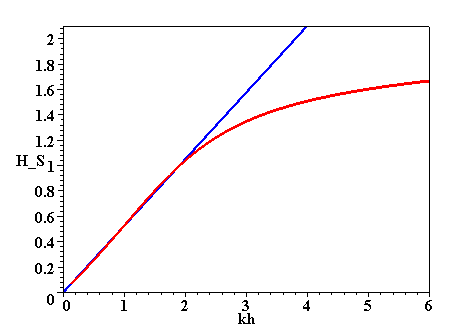
\includegraphics[scale = 0.8]{HSkh.png}
\end{center}
\caption[A graph for the ratios between the wave height $H$ and the stroke $S$ with respect to the relative depth $k_{p}\,h$.]{A graph for the ratios between the wave height $H$ and the stroke $S$ with respect to the relative depth $k_{p}\,h$. The horizontal axis label \textbf{kh} refers to $k_{p}\,h$, while the vertical axis label \textbf{H\_S} refers to $H/S$.}			\label{gambar1}
\end{figure}

% Chapter 4
\chapter{Numerical Simulation}  \label{numeric}

In this chapter, we will discuss several results by selecting particular values from the wave-related quantities.
Using the computer software \emph{Maple V Release 5}, we could also observe an animation for the resulting monochromatic waves when we move the wavemaker with a particular stroke.

% Section 4.1
\section{Calculating the Progressive Wavenumber} 		\label{NR1}

Consider again equation~\eqref{progresif} which expresses the dispersion relationship for progressive waves
\begin{equation}
\omega^2 = g\,k_{p}\: \tanh\: k_{p}\,h.
\end{equation}
Since we are not able to calculate the exact value of the wavenumber $k_p$, we need to calculate it numerically. We use the following values: monochromatic frequency $\omega = 2$~rad/s, gravitational acceleration constant $g = 9.8$~m/s$^2$, and the water depth of the towing tank $h = 3$~m. Employing the Newton-Raphson iteration, we seek the value $k_p$ given an initial guess $p_0$ by finding the roots of $f(k_{p}) = 0$, where $f(k_{p}) = \omega^2 - g\, k_{p} \: \tanh \: k_{p} \, h$. Please see Appendix~B for more information on the algorithm for the Newton-Raphson iteration. By choosing error values of $\delta = 10^{-9}$, $\epsilon = 10^{-9}$, and {\ttfamily small} $= 10^{-9}$, as well as the maximum iteration $= 5000$, then using the initial guess $p_{0} = 0.5$, we obtain $k_{p} = 0,4624593666$. For $\omega = 1$, the obtained value for the progressive wavenumber is $k_{p} = 0,1943823443$. See again the graph in Figure~\ref{gambar2}.

% Section 4.2
\section{Calculating Standing Wave Wavenumbers} \label{NR2}

Consider again equation~\eqref{berdiri} which expresses the dispersion relationship for standing waves
\begin{equation}
\omega^2 = -g \, k_{s} \: \tan \: k_{s} \,h.
\end{equation}
Similar as previously, since we cannot calculate exact values of the wavenumber $k_s$, we calculate them numerically. We take identical values as previously: monochromatic frequency $\omega = 2$~rad/s, gravitational acceleration constant $g = 9.8$~m/s$^2$, and the water depth of the towing tank $h = 3$~m. Employing the Newton-Raphson iteration, we seek the values $k_s$ given an initial guess $p_0$ by finding the roots of $g(k_{s}) = 0$, where $g(k_{s}) = \omega^2 + g \, k_{s} \: \tan \: k_{s}\,h$. Please consult Appendix~B for more detailed information on the algorithm for the Newton-Raphson iteration. The selected error values are $\delta = 10^{-5}$, $\epsilon = 10^{-5}$, and {\ttfamily small} $= 10^{-5}$ with the maximum iteration of 10000. Since the graph in the dispersion relationship produces infinitely many intersections, i.e., the values of standing wave wavenumbers, then the values for an initial guess also vary according to the computational need, $p_{0} = 1, 2, 3, \cdots$. For a practical purpose, we only select several successive wavenumber values, given as follows:
\begin{align*}
k_{s}(1) &= 0.906121231; \\
k_{s}(2) &= 2.028197863;  \\
k_{s}(3) &= 3.097926261;  \\
k_{s}(4) &= 4.156159228;  \\
k_{s}(5) &= 5.209926525;  \\
k_{s}(6) &= 6.261487236;  \\
k_{s}(7) &= 7.311794624;  \\
k_{s}(8) &= 8.361321437;  \\
k_{s}(9) &= 9.410329031.
\end{align*}
See again the graph in Figure~\ref{gambar3}.

Similarly, using various values for the initial guess, we obtain the following wavenumber values corresponding to the standing waves for $\omega = 1$:
\begin{align*}
k_{s}(1) &= 1.013758189;	\\
k_{s}(2) &= 2.078040121;	\\
k_{s}(3) &= 3.130732073;	\\
k_{s}(4) &= 4.180655871.
\end{align*}

% Section 4.3
\section{Monochromatic Wave Profiles}

% Subsection 4.3.1
\subsection{Two Wave Profiles with Distinct Wave Height $H$}

Consider again the velocity potential equation~\eqref{lastpotensial} describing a water wave produced by the wavemaker
\begin{align}
\phi(x,\,z,\,t) &= A_{p} \: \cosh \, k_{p} \, (h + z) \: \sin \, (k_{p}\,x - \omega\,t) \nonumber \\
& \quad + \, \sum_{n=1}^{\infty} C_{n} \: e^{-k_{s}(n) \, x} \: \cos \, k_{s}(n) \, (h + z) \: \cos (\omega \,t).
\end{align}
Using equations~\eqref{firstconst} and~\eqref{ratio}, we can express the coefficient $A_p$ in terms of $\omega$, $H$, $k_{p}$, and $h$, i.e.,
\begin{equation}
A_{p} = \frac{\omega \, H}{2 \, k_{p} \: \sin \: k_{p}\,h}.
\end{equation}
By substituting the values $\omega = 2$, $k_{p} = 0,4624593666$, and $h = 3$, then
\begin{itemize}[leftmargin=1.2em]
\item for $H = 0.5 $, we have $A_{p} = 1.099621133$; and
\item for $H = 0.75$, we have $A_{p} = 1.649431700$.
\end{itemize}

To obtain the maximum stroke $S$, we use equation~\eqref{ratio}, i.e.,
\begin{equation}
S = \left(\frac{H \, k_{p} \, h}{4 \, \sinh \, k_{p} \, h} \right) \; 
\left(\frac{\sinh \, 2 \, k_{p} \, h + 2 \, k_{p} \, h}{k_{p} \,h \: \sinh \, k_{p} \, h - \cosh \, k_{p} \, h + 1} \right).
\end{equation}
Substituting the values we have chosen, it yields
\begin{itemize}[leftmargin=1.2em]
\item for $H = 0.5 $, we obtain $S = 0.2908632665$; and
\item for $H = 0,75$, we obtain $S = 0.4362948995$.
\end{itemize}

The wavemaker movement profile when it reaches the maximum stroke can be viewed in Figure~\ref{gambar4}.~
\begin{figure}[!htbp]
\begin{center}
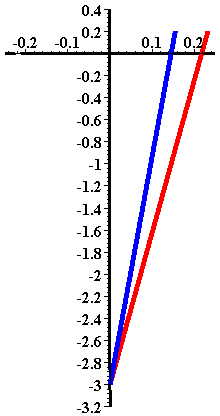
\includegraphics[scale = 0.7]{flap1.png}
\end{center}
\caption{Maximum strokes from the wavemaker flap which produce two wave-profiles with different wave height.}	\label{gambar4}
\end{figure}

To find the coefficients for the standing wave $C_n$, we use~\eqref{nextconst}, namely
\begin{equation}
C_{n} = \frac{-2 \, \omega \, S}{[k_{s}(n)]^2 \, h} \; \frac{[k_{s}(n) \, h] \: \sin \, [k_{s}(n) \, h] 
+ \cos \, [k_{s}(n) \, h]}{\sin \, [2 \, k_{s}(n) \,h ] + 2 \, k_{s}(n) \,h}.
\end{equation}
We have already selected four values of $k_{s}(n)$. For larger values of $n$, the effect of $C_n$ to the wave profile solution is relatively small so that it can be neglected.
\begin{itemize}[leftmargin=1.2em]
\item For $S = 0.2908632665$, the coefficient values are \ $C_{1} = 0.08013595964$, $C_{2} = 0.00976252019$, $C_{3} = 0.001714039296$, and $C_{4} = 0.001110132786$.
\item For $S = 0.4362948995$, the coefficient values are \ $C_{1} = 0.1202039395 $, $C_{2} = 0.01464378027$, $C_{3} = 0.002571058938$, and $C_{4} = 0.001665199177$.
\end{itemize}

Using equation~\eqref{permukaan}
\begin{equation}
\eta(x,\,t) = -\frac{1}{g} \: \left. \left(\frac{\partial \phi}{\partial t} \right) \right|_{z = 0}
\end{equation}
we are able to discover an equation for the shape of the formed water wave elevation. We can also display this surface elevation using computer software. The simulation result for the water surface with two distinct wave heights is displayed in Figure~\ref{gambar5}.
\begin{figure}[h]
\begin{center}
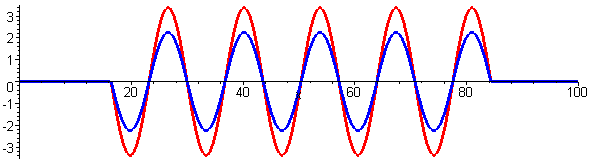
\includegraphics[scale = 0.8]{elevasi1.png}
\end{center}
\caption{Shapes of surface water wave elevation for two distinct wave heights.} 	\label{gambar5}
\end{figure}

\subsection{Two Wave Profiles with Distinct Angular Frequency $\omega$}

In this subsection, we implement an identical technique as in the previous subsection. The water depth in the towing tank is also $h = 3$~m and the desired wave height profile is $H = 0.5$~m. The angular frequencies are $\omega = 2$ and $\omega = 1$. Employing the Newton-Raphson iteration toward both the progressive wave and the standing wave dispersion relationships, we could attain the values $k_{p}$ and $k_{s}(n)$ for these frequencies. We have obtained these results in Sections~\ref{NR1} and~\ref{NR2}. We tabulate them again in this section. Additionally, we also list the coefficients for the velocity potential related to the values of $\omega$, i.e., $A_{p}$ and $C_{n}$. 

The following provides results obtained by the computer software \emph{Maple V Release 5}.
\begin{description}[leftmargin=1.3em]
\item[\textbf{a.}]  For $\omega = 2$.
\begin{itemize}[leftmargin=0.8em]
\item A wavenumber for the progressive wave $k_{p} = 0.4624593666$.

\item Wavenumbers for the standing wave:\\
\hspace*{1em} $k_{s}(1) = 0.9061212307$, \qquad \qquad $k_{s}(2) = 2.028197863$, \\
\hspace*{1em} $k_{s}(3) = 3.0979262610$, \qquad \qquad $k_{s}(4) = 4.156159228$.

\item The coefficient $A_{p} = 1.099621133$.

\item The maximum stroke $S = 0.2908632665$.

\item The coefficients $C_{n}$ are \\
\hspace*{1em} $C_{1} = 0.801359596400$, \qquad \qquad $C_{2} = 0.009762520190$, \\
\hspace*{1em} $C_{3} = 0.001714039296$, \qquad \qquad $C_{4} = 0.001110132786$.
\end{itemize}

\item[\textbf{b.}] For $\omega = 1$.
\begin{itemize}[leftmargin=0.8em]
\item A wavenumber for the progressive wave $k_{p} = 0.1943823443$.

\item Wavenumbers for the standing wave: \\
\hspace*{1em} $k_{s}(1) = 1.013758189$, \qquad \qquad $k_{s}(2) = 2.078040121$, \\
\hspace*{1em} $k_{s}(3) = 3.130732073$, \qquad \qquad $k_{s}(4) = 4.180655871$.

\item The coefficient $A_{p} = 2.335633604$.

\item The maximum stroke $S = 1.140576790$.

\item The coefficients $C_{n}$ are \\
\hspace*{1em} $C_{1} = 0.212585384200$, \qquad \qquad $C_{2} = 0.0043694275640$, \\
\hspace*{1em} $C_{3} = 0.007018430814$, \qquad \qquad $C_{4} = 0.0005323318426$.
\end{itemize}
\end{description}
The flap deviation profile for the maximum strokes is displayed in Figure~\ref{gambar6}.
The wave profiles evolution in time is presented in Figures~\ref{gambar7}--\ref{gambar14}.
\begin{figure}[h]
\begin{center}
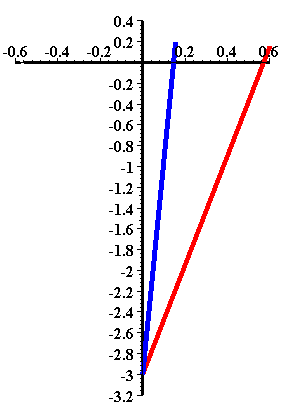
\includegraphics[scale = 0.8]{flap2.png}
\end{center}
\caption{The maximum strokes from the flap which produce two wave-profiles with distinct frequency.}   		\label{gambar6}
\end{figure}
\newpage
\begin{figure}[h]
\begin{center}
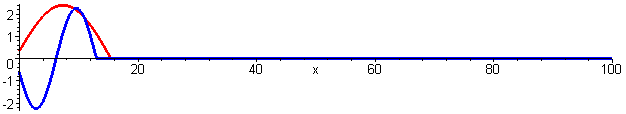
\includegraphics[scale = 0.8]{animasi3.png}
\end{center}
\caption{Water wave surface graphs at $t = 3$.}   \label{gambar7}
\end{figure}
\vfill
\begin{figure}[h]
\begin{center}
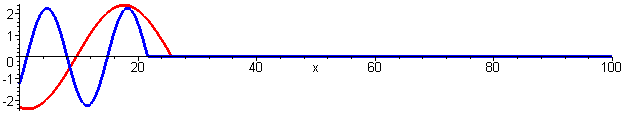
\includegraphics[scale = 0.8]{animasi5.png}
\end{center}
\caption{Water wave surface graphs at $t = 5$.}   \label{gambar8}
\end{figure}
\vfill
\begin{figure}[h]
\begin{center}
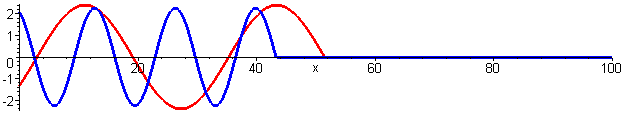
\includegraphics[scale = 0.8]{animasi10.png}
\end{center}
\caption{Water wave surface graphs at $t = 10$.}  \label{gambar9}
\end{figure}
\vfill
\begin{figure}[b!]
\begin{center}
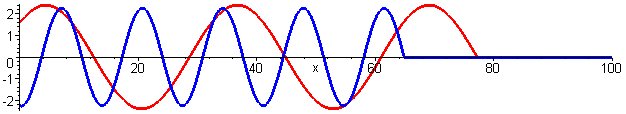
\includegraphics[scale = 0.8]{animasi15.png}
\end{center}
\caption{Water wave surface graphs at $t = 15$.}  \label{gambar10}
\end{figure}
\newpage
\begin{figure}[h]
\begin{center}
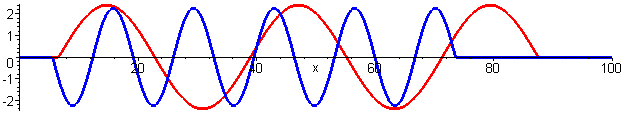
\includegraphics[scale = 0.8]{animasi17.png}
\end{center}
\caption{Water wave surface graphs at $t = 17$.}   \label{gambar11}
\end{figure}
\vfill
\begin{figure}[h]
\begin{center}
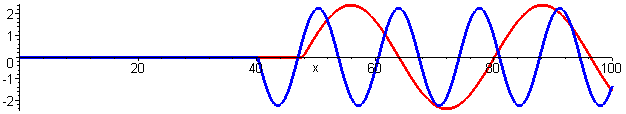
\includegraphics[scale = 0.8]{animasi25.png}
\end{center}
\caption{Water wave surface graphs at $t = 25$.}   \label{gambar12}
\end{figure}
\vfill
\begin{figure}[h]
\begin{center}
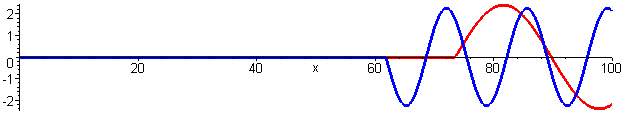
\includegraphics[scale = 0.8]{animasi30.png}
\end{center}
\caption{Water wave surface graphs at $t = 30$.}   \label{gambar13}
\end{figure}
\vfill
\begin{figure}[b!]
\begin{center}
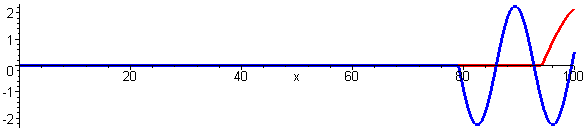
\includegraphics[scale = 0.8]{animasi34.png}
\end{center}
\caption{Water wave surface graphs at $t = 34$.}   \label{gambar14}
\end{figure}

% Chapter 5
\chapter{Conclusion and Suggestion}

% Section 5.1
\section{Conclusion}

The following presents conclusion for this final project report:
\begin{itemize}[leftmargin=1.5em]
\item[\textbf{a.}] We have adopted ideal fluid assumptions for wave generation modeling.
\item[\textbf{b.}] We have implemented linear wave theory for solving the governing differential equations obtained from part (a).
\item[\textbf{c.}] We were able to derive the relationship among the wavenumber, wave height, and wavemaker stroke from the theory developed in part (b).
\item[\textbf{d.}] For shallow-water waves, both the simplified and the linear wave theories produce an identical result, while for deeper-water waves, both theories provide different results.
\end{itemize}

% Section 5.2
\section{Suggestion}

The following presents suggestion for another final project or further research: 
\begin{itemize}[leftmargin=1.5em]
\item[\textbf{a.}] The wave theory can be extended to nonlinear theory and three-dimensional wavemaker theory.
\item[\textbf{b.}] The type of waves can be expanded to include random and irregular waves.
\item[\textbf{c.}] Adding a beach can be utilized to replace a semi-infinite domain.
\end{itemize}

% Appendices
\appendix

% Appendix A
\chapter{Material Derivative}

The operator
\begin{equation}
\frac{\mathrm{D}}{\mathrm{D}t} = \frac{\partial}{\partial t} + \mathbf{u}\cdot \nabla  			\label{op}
\end{equation}
is known as the material derivative, total derivative, substantial derivative, or Lagrange derivative. In general $\displaystyle \frac{\mathrm{D}}{\mathrm{D}t}$ is a vector operator. As a consequence, $\displaystyle \frac{\mathrm{D}}{\mathrm{D}t}$ components acts on a vector will not be equal with the ones act on a scalar component of a vector, except in the Cartesian coordinates system. The material derivative can also be applied to a scalar quantity, such as temperature. Physically, it states the rate of change of that quantity with respect to time, where the observer moves along with the measured fluid at a particular location in space and instant time when that derivative is evaluated.

This operator is the total derivative with respect to time acting on a fluid element, which can be viewed as follows. Let $\xi$ be a spatial coordinate describing the fluid at an initial fixed instant $t = 0$, let also $\mathbf{x}$ be the spatial coordinate providing the location during time $t$ of a fluid element for which it is $\xi$ when $t = 0$. We have $\mathbf{x} = \mathbf{x}(\xi,\tau)$. The Eulerian derivative with respect to time is given by
\begin{equation}
\frac{\partial}{\partial t} = \left. \frac{\partial}{\partial t} \right|_{\text{fixed} \; \mathbf{x}},
\end{equation}
while the derivative which plays a role as Lagrangian derivative is given by
\begin{equation}
\frac{\mathrm{D}}{\mathrm{D}t} = \left. \frac{\partial}{\partial t}\right|_{\text{fixed} \; \xi}.
\end{equation}
Employing the Chain Rule, we obtain
\begin{equation*}
\frac{\mathrm{D}}{\mathrm{D}t} 
= \left. \frac{\partial}{\partial t} \right|_{\text{fixed} \; \xi} 
= \left. \frac{\partial}{\partial t} \right|_{\text{fixed} \; \mathbf{x}} + 
  \left. \frac{\partial x_i}{\partial t} \right|_{\text{fixed} \; \xi} \frac{\partial}{\partial t},
\end{equation*}
which results equation~\eqref{op} since $\displaystyle \left. \frac{\partial \mathbf{x}}{\partial t} \right|_{\xi} = \mathbf{u}$.

This operator is also used in the Navier-Stokes equation which states the total acceleration of a particle as follows:
\begin{equation}
\mathbf{a} = \frac{\mathrm{D}\mathbf{u}}{\mathrm{D}t} = 
\frac{\partial \mathbf{u}}{\partial t} + \left(u \frac{\partial \mathbf{u}}{\partial x} + v \frac{\partial \mathbf{u}}{\partial y} + 
w \frac{\partial \mathbf{u}}{\partial z} \right).  			\label{nv}
\end{equation}
The first term on the right-hand side of~\eqref{nv} indicates a local acceleration, which is zero for the steady-state flow. The other terms express convective acceleration, which show that the fluid flow has a different velocity at a different position. For more detailed explanation, please consult~\cite{fac,hwf}.

% Appendix B
\chapter[Newton-Raphson Iteration]{An Algorithm for the Newton-Raphson Iteration}

%\fbox{\begin{minipage}{16cm} \vspace*{0.5cm}

\ovalbox{
\begin{minipage}{15.0cm}
\vspace{0.5cm}
\bfseries Searching the root of $f(x) = 0$ given an initial guess $p_0$ using the iteration\newline $\displaystyle p_{n} = p_{n - 1} - \frac{f(p_{n - 1})}{f'(p_{n - 1})}$ for $n = 1, 2, 3, \dots$. \vspace{0.5cm}
\end{minipage}
} 
\vspace{0.5cm} \\
\textbf{Algorithm:}\\
{\ttfamily $\delta:= 10^{-6}$, \qquad $\epsilon:= 10^{-6}$, \qquad small$:= 10^{-6}$ \\
\{ several error values, can be adjusted according to the need \} \\
maks$:= 99$ \qquad \qquad \{ the maximum number of iterations \} \\
kond$:=  0$ \qquad \qquad \{ the condition for a loop termination \} \\
INPUT $P_0$ \qquad \qquad \{ $P_0$ must be sufficiently close with the desired root \} \\
$Y_0:=F(P_0)$ \qquad \qquad \{ calculating a value of the function \} \\
\newline
DO FOR $N:= 1$ TO maks UNTIL kond $\neq$ 0 \\
\hspace*{.2in} $Df:= F^{\prime}(P_0)$ \qquad \qquad \{ calculating the derivative \} \\
\hspace*{.5in} IF $Df = 0$ THEN \qquad \qquad 	\\	\{ checking whether there exists any division by zero \} \\
\hspace*{1in} kond$:= 1$ \\
\hspace*{1in} $Dp:= 0$ \\
\hspace*{.8in} ELSE \\
\hspace*{1in} $Dp:= Y_0/Df$ \\
\hspace*{.5in} ENDIF \\
\hspace*{.2in} $P_1:= P_0 - Dp$ \qquad \qquad \{ new iteration \} \\
\hspace*{.2in} $Y_1:= F(P_1)$   \qquad \qquad \{ the value of a new function \} \\
\hspace*{.2in} RelErr$:= 2\ast|Dp|/(|P1| + \texttt{small})$ \qquad \qquad \{ relative error \} \\
\hspace*{.2in} IF RelErr $< \delta$ AND $|Y_1| < \epsilon$ THEN \\
\hspace*{.5in} IF kond $\neq$ 1 THEN kond$:= 2$ \qquad \qquad \{ checking convergence \}  \\
\hspace*{.2in} $P_0:= P_1$; \qquad $Y_0:= Y_1$  \qquad \qquad \{ replacing with new values \} \\
\newline
PRINT `The value of the $n$-th iteration is' $P_1$ \qquad \qquad \{ ouput \} \\
PRINT `The successive iteration differs by' $Dp$  \\
PRINT `The value of $f(x)$ is' $Y1$ \\
IF kond$= 0$ THEN \\
\hspace*{.2in} PRINT `The number of maximum iteration has been exceeded.' \\
IF kond$= 1$ THEN \\
\hspace*{.2in} PRINT `There exists a division by zero.' \\
IF kond$= 2$ THEN \\
\hspace*{.2in} PRINT `A root has been found with the desired error.'
}

% Appendix C
\chapter[Hydrodynamics Laboratories]{Hydrodynamics Laboratories Around the World}

This appendix lists hydrodynamic laboratories in various parts of the world. Some of them are used commercially and for marine structure defense. For detailed information, please consult~\cite{csk} or the International Towing Tank Conference association. Otherwise indicated, the size of the tank refers to the length, width, and depth, respectively.
\vfill
\begin{itemize}[leftmargin=1.5em]
\item[\textbf{a.}] Institute of Marine Dynamics Towing Tank, St. John's, Newfoundland, Canada \\
\begin{tabular}{@{}ll}
Facility: & Deep-water tank \\
Tank size:& 200~m $\times$ 12~m $\times$ 7~m \\
Carrier speed:& 10 m/s \\
Wave type:& Regular and irregular; 1~m \\
Wavemaker:& Double flap-type \\
Beach:& Surging wave bottom.
\end{tabular}
\vfill

\item[\textbf{b.}] Offshore Model Basin, Escondido, California, United States (US) \\
\begin{tabular}{@{}ll}
Tank size:& 90~m $\times$ 14.6~m $\times$ 4.6~m \\
Deeper part:& Circular hole with 9~m depth \\
Carrier speed:& 6 m/s \\
Wave type:& Regular and irregular; 0.74~m \\
Wavemaker:& Single-flap board \\
Beach:& Metal shaved.
\end{tabular}
\vfill

\item[\textbf{c.}] Offshore Technology Research Center, Texas A\&M, College Station, Texas, US \\
\begin{tabular}{@{}ll}
Tanks size:& 45.7~m $\times$ 30.5~m $\times$ 5.8~m \\
Deeper part:& 16.7~m hole with adjustable floor \\
Wavemaker:& Flap-type with hydraulic hinge control \\
Maximum wave height:& 80~cm \\
Period range:& 0.5--4.0~s \\
Beach:& Metal panel
\end{tabular}

\item[\textbf{d.}] David Taylor Research Center, Bethesda, Maryland, US \\
\begin{tabular}{@{}ll}
Facility:& Maneuvering and Seakeeping Facilities (MASK) \\
Tank size:& 79.3~m $\times$ 73.2~m $\times$ 6.1~m \\
Wavemaker:& Total of 21 pneumatic-type \\
Wave:& Multidirectional, regular and irregular; maximum height 0.6~m;\\
     & and wavelength 0.9--12.2~m \\
Beach:& Wave absorber \\
Carrier speed:& 7.7 m/s.
\end{tabular}

\begin{tabular}{@{}ll}
Facility:& Deep-Water Basin \\
Tank size:& 846~m $\times$ 15.5~m $\times$ 6.7~m \\
Wave:& Maximum height 0.6~m and wavelength 1.5--12.2~m \\
Carrier speed:& 10.2 m/s. 
\end{tabular}

\begin{tabular}{@{}ll}
Facility:& High-Speed Basin \\
Tank size:& 79.3~m $\times$ 73.2~m $\times$ 6.1~m \\
Wave:& Maximum height 0.6~m and wavelength 0.9--12.2~m \\
Carrier speed:& 35.8--51.2 m/s.
\end{tabular}

\item[\textbf{e.}] Maritime Research Institute (MARIN), the Netherlands \\
\begin{tabular}{@{}ll}
Facility:& Seakeeping Basin \\ 
Tank size:& 100~m $\times$ 24.5~m $\times$ 2.5~m \\
Deeper part:& Hole with 6~m depth \\
Wave:& Regular and irregular; maximum height 0.3~m; and period range 0.7--3.0~s \\
Carrier speed:& 4.5 m/s.
\end{tabular}

\begin{tabular}{@{}ll}
Facility:& Wave and Current Basins \\
Tank size:& 60~m $\times$ 40~m $\times$ 1.2~m \\
Deeper part:& Hole with 3~m depth \\
Wave:& Regular and irregular \\
Carrier speed:& 3 m/s \\
Speed range:& 0.1--0.6 m/s.
\end{tabular}

\begin{tabular}{@{}ll}  
Facility:& Deep-Water Towing Tank \\
Tank size:& 252~m $\times$ 10.5~m $\times$ 5.5~m \\
Carrier speed:& 9 m/s.
\end{tabular}

\begin{tabular}{@{}ll}
Facility:& High-Speed Towing Tank \\
Tank size:& 220~m $\times$ 4~m $\times$ 4~m \\
Wavemaker:& Hydraulic flap-type \\
Wave:& Regular and irregular; maximum height 0.4~m; and period range 0.3--5~s \\
Carrier:& Motor and jet controls \\
Carrier speed:& 15~m/s and 30~m/s \\
Beach:& Circular arc lattices.
\end{tabular}

\item[\textbf{f.}] Danish Maritime Institute, Lyngby, Denmark \\
\begin{tabular}{@{}ll}
Tank size:& 240~m $\times$ 12~m $\times$ 5.5~m \\
Wavemaker:& Hydraulic double-flap type controlled numerically \\
Wave:& Regular and irregular; maximum wave 0.4~m; and period range 0.5--7~s \\
Carrier speed:& 0--11 m/s (accurate $\pm$ 2\%).
\end{tabular}

\item[\textbf{g.}] Danish Hydraulic Institute, Horsholm, Denmark \\
\begin{tabular}{@{}ll}
Tank size:& 30~m $\times$ 20~m $\times$ 3~m \\
Deeper part:& 12~m in the middle \\
Wavemaker:& 60 Hydraulic flaps controlled by a mini-computer on one side \\
Wave:& Maximum height $\cong$ 0.6~m and period range $\cong$ 0.5--4~s.
\end{tabular}

\item[\textbf{h.}] Norwegian Hydrodynamic Laboratory (MARINTEK), Trondheim, Norway \\
\begin{tabular}{@{}ll}
Facility:& The Ocean Basin \\
Tank size:& 80~m $\times$ 50~m $\times$ 10~m \\
Wavemaker:& Hinged double-flap type, 144 self-control; Hydraulic controlled hinge-type \\
Wave:& Regular and irregular; maximum height 0.9~m \\
Wave speed:& Maximum speed 0.2 m/s.
\end{tabular}
\end{itemize}

% References
\begin{thebibliography}{99}
\bibitem{aph}  \textbf{Azoury, P. H.,} Engineering Applications of Unsteady
Fluid Flow, John Wiley \& Sons, 1992. (ISBN 0 471 92968 9; 97/602; 620.1'064
AZO). \addcontentsline{toc}{chapter}{References}

\bibitem{csk}  \textbf{Chakrabarti, S. K.,} Offshore Structure Modelling,
World Scientific, 1994. (ISBN 981-02-1513-4; 96/5715; 627.98 CHA)

\bibitem{drg}  \textbf{Dean, R. G., Dalrymple, R. A.,} Water Wave Mechanics
for Engineers and Scientists, World Scientific, 1991. (ISBN
9810204205-9810204213; 627'.042-dc20)

\bibitem{dmw}  \textbf{Dingemans, M. W.} Water Wave Propagation Over Uneven
Bottoms, Part 1 - Linear Wave Propagation, World Scientific, 1997. (ISBN
981-02-3393-9)

\bibitem{fac}  \textbf{Fowler, A. C., } Mathematical Models in the Applied
Sciences, Cambridge University Press, 1997.

\bibitem{gev}  \textbf{Groesen, E. van,} Lecture Notes Computational Fluid
Dynamics, Research Workshop, University of Twente, 1997.

\bibitem{hjp}  \textbf{Hooft, J. P.,} Advanced Dynamics of Marine
Structures, John Wiley \& Sons, 1982. (ISBN 0-471-03000-7; 87/2262; 627'.042
HOO)

\bibitem{hwf}  \textbf{Hughes, W. F., Brighton, J. A.,} Theory and Problems
of Fluid Dynamics, $2^\text{nd}$ Edition, Schaum's Outline Series, McGraw--Hill,
Inc., 1991. (ISBN 0-07-112632-5; 94/501; 532-05 HUG)

\bibitem{jrs}  \textbf{Johnson, R. S.,} A Modern Introduction to the
Mathematical Theory of Water Waves, Cambridge University Press, 1997 (ISBN 0
521 59832 X)

\bibitem{kjp}  \textbf{Keener, J. P.,} Principles of Applied Mathematics ---
Transformation and Approximation, Addison--Wesley Publishing Company, 1988.

\bibitem{lld}  \textbf{Landau, L. D., Lifshitz, E. M.,} Fluid Mechanics (%
\textit{Mekhanika Sploshnykh Sred}), $2^\text{nd}$ English Edition, Volume 6 of
Course of Theoretical Physics (\textit{Teoreticheska$\widehat{ia}$ Fizika}),
Translated from the Russian by J. B. Sykes and W. H. Reid, Pergamon Press,
1987.

\bibitem{mjh}  \textbf{Mathews, J. H.,} Numerical Methods for Mathematics,
Science, and Engineering, $2^\text{nd}$ Edition, Prentice-Hall, 1992. (ISBN
0-13-624990-6)

\bibitem{njn}  \textbf{Newman, J. N.,} Marine Hydrodynamics, MIT Press,
1977. (ISBN 0-262-14026-8)

\bibitem{rs}  \textbf{Ramamrutham, S.,} Fluid Mechanics, Hydraulics, and
Fluid Machines, Dhanpat Rai \& Sons, 1986. (90/522; 620.106 RAM)

\bibitem{rgf}  \textbf{Round, G. F., Garg, V. K.,} Applications of Fluid
Dynamics, Edward Arnold, 1986. (ISBN 0-7131-3546-8; 87/1153; 620.1'064 ROU)

\bibitem{tgb}  \textbf{Thomas, Jr. G. B., Finney, R. L.,} Calculus and
Analytic Geometry, $9^\text{th}$ Edition, Addison--Wesley Publishing Company,
1996. (ISBN 0-201-40015-4; 515.15 THO; 08119)

\bibitem{wlh}  \textbf{Wiryanto, L. H.,} Lecture Notes MA-475 Computational Fluid Dynamics (in Indonesian), Department of Mathematics, Faculty of Mathematics and Natural Sciences, Bandung Institute of Technology, 2000.
\end{thebibliography}
\end{document}
